\documentclass[12pt,a4paper]{article}
\usepackage[T1]{fontenc}
\usepackage{amsmath}
\usepackage{newtxtext,newtxmath}
\usepackage[left=3cm,right=2.5cm,top=2.5cm,bottom=2.5cm,footskip=0.6cm]{geometry}
\usepackage{graphicx,calc}
\usepackage{setspace,eso-pic,tikz,array,booktabs,enumitem,caption,titlesec,fancyhdr,tocloft,float}
\usepackage[hidelinks]{hyperref}
\usetikzlibrary{arrows.meta,positioning,shapes.geometric,fit,backgrounds}
\onehalfspacing
\setlength{\parindent}{0pt}\setlength{\parskip}{6pt}

% single-line page border on every page (title page included)
\AddToShipoutPictureBG{%
  \AtPageLowerLeft{\put(\LenToUnit{1.5cm},\LenToUnit{1.5cm}){%
    \framebox(\LenToUnit{\paperwidth-3cm},\LenToUnit{\paperheight-3cm}){}}}}
\setlength{\fboxrule}{0.8pt}

\titleformat{\section}{\fontsize{14}{17}\bfseries}{\thesection.}{0.6em}{}
\titleformat{\subsection}{\normalsize\bfseries}{\thesubsection}{0.6em}{}
\titleformat{\subsubsection}{\normalsize\itshape}{\thesubsubsection}{0.6em}{}
\titlespacing*{\section}{0pt}{12pt}{6pt}
\titlespacing*{\subsection}{0pt}{10pt}{4pt}
\captionsetup{font=small,labelfont=bf}
\fancypagestyle{plain}{\fancyhf{}\fancyfoot[C]{\thepage}\renewcommand{\headrulewidth}{0pt}}
\pagestyle{plain}
\renewcommand{\cftsecleader}{\cftdotfill{\cftdotsep}}
\renewcommand{\contentsname}{Index}
\newcolumntype{P}[1]{>{\raggedright\arraybackslash}p{#1}}
\newcolumntype{C}[1]{>{\centering\arraybackslash}p{#1}}

\begin{document}
% ------------------------------------------------------------------ TITLE PAGE (common format)
\begin{titlepage}
\centering
\vspace*{-0.8cm}

\includegraphics[width=0.46\linewidth]{upes_logo.png}\\[0.4cm]
{\large\bfseries School of Computer Science, UPES, Dehradun}\\[0.8cm]
{\large A Project Report on}\\[0.5cm]
{\fontsize{19}{24}\selectfont\bfseries Hospital Delivery Robot with Probabilistic\\[3pt] Roadmap (PRM)\par}
\vspace{0.7cm}
{\normalsize Submitted for the course}\\[4pt]
{\large\bfseries CSAI4014 Algorithms for Intelligent Systems and Robotics}\\[4pt]
B.Tech CSE (AI \& ML), Semester VII\\[0.6cm]
\begin{tabular}{ll}
\textbf{Project No.:} & P05 \\
\textbf{Group No.:} & G01 \\
\textbf{Batch:} & B3 \\
\end{tabular}\\[0.5cm]
{\bfseries Submitted by}\\[4pt]
\renewcommand{\arraystretch}{1.15}
\begin{tabular}{|c|P{6.2cm}|c|}
\hline
\textbf{S. No.} & \textbf{Name} & \textbf{SAP ID} \\ \hline
1 & Supreet Kaur & 500122005 \\ \hline
2 & Aditi Verma & 500123675 \\ \hline
3 & Parag Goyal & 500124297 \\ \hline
4 & Kushal Gupta & 500121188 \\ \hline
5 & Aman Rathore & 500122510 \\ \hline
\end{tabular}\\[0.6cm]
{\bfseries Submitted to}\\[2pt]
Course Faculty, CSAI4014\\
School of Computer Science, UPES, Dehradun\\[0.6cm]
{\bfseries Academic Year 2026-2027 \quad | \quad October 2026}
\end{titlepage}

% ------------------------------------------------------------------ FRONT PAGES (Roman numbers)
\pagenumbering{roman}\setcounter{page}{1}

% DECLARATION
\section*{Declaration}
\addcontentsline{toc}{section}{Declaration}
We declare that this project report titled ``Hospital Delivery Robot with Probabilistic Roadmap (PRM)'' is our own work, carried out for the course CSAI4014 Algorithms for Intelligent Systems and Robotics. The code, results, analysis, and text are original, and all sources used have been cited in the References.

\vspace{0.8cm}
\begin{table}[h]
\centering
\resizebox{\linewidth}{!}{%
\renewcommand{\arraystretch}{2.0}
\begin{tabular}{|P{5.2cm}|P{3.2cm}|P{4.8cm}|}
\hline
\textbf{Name} & \textbf{SAP ID} & \textbf{Signature} \\ \hline
Supreet Kaur & 500122005 & \\ \hline
Aditi Verma & 500123675 & \\ \hline
Parag Goyal & 500124297 & \\ \hline
Kushal Gupta & 500121188 & \\ \hline
Aman Rathore & 500122510 & \\ \hline
\end{tabular}%
}
\end{table}

\vspace{0.8cm}
Date: \rule{4cm}{0.4pt} \hfill Place: Dehradun
\newpage

% ABSTRACT & KEYWORDS
\section*{Abstract}
\addcontentsline{toc}{section}{Abstract}
Autonomous mobile service robots deployed in modern healthcare facilities must reliably transport pharmaceuticals, sterile lab specimens, and supplies between a central pharmacy and multiple inpatient wards across structured indoor floors. This project presents \textbf{MediRoute}, a multi-query autonomous delivery robot system combining a specialized Probabilistic Roadmap (PRM) motion planner with dynamic replenishment, closed-loop heading feedback control, and priority mission scheduling. To overcome the classical ``narrow passage problem'' where standard uniform PRM sampling fails to connect narrow doorways, we implement a targeted door-biased sampling scheme that injects localized candidate nodes into doorway bounding boxes. The architecture integrates an adaptive roadmap refresh routine that repairs graph edges without discarding valid vertices when dynamic corridor obstacles appear, alongside an energy-aware mission executive with automated charging-dock diversion. Evaluated across 10-trial Monte Carlo experiments, the door-biased PRM achieves a 100\% planning success rate even under constricted door clearances down to 0.65\,m (where uniform PRM drops to 3.3\%), and yields a $12.95\times$ computational speedup through roadmap reuse compared to repeated single-query rebuilding. Complete multi-ward missions execute without collision across simulated dynamic events.

\vspace{0.4cm}
\textbf{Keywords:} mobile robot, Probabilistic Roadmap (PRM), hospital delivery, motion planning, door-biased sampling, narrow passage, differential-drive control, OMPL, CoppeliaSim.
\newpage

% TABLE OF CONTENTS (INDEX)
\tableofcontents
\newpage

% LIST OF FIGURES & LIST OF TABLES
\listoffigures
\addcontentsline{toc}{section}{List of Figures}
\vspace{0.8cm}
\listoftables
\addcontentsline{toc}{section}{List of Tables}
\newpage

% WRITING ALLOCATION
\section*{Writing Allocation}
\addcontentsline{toc}{section}{Writing Allocation}
In accordance with course guidelines, the technical authorship of this report has been divided equally among all five team members. Table~\ref{tab:writing_allocation} outlines the specific writing allocation.

\begin{table}[h]
\centering
\caption{Report Writing Allocation among Team Members}
\label{tab:writing_allocation}
\resizebox{\linewidth}{!}{%
\renewcommand{\arraystretch}{1.3}
\begin{tabular}{|c|P{4.6cm}|P{5.6cm}|c|}
\hline
\textbf{Member} & \textbf{Name and SAP ID} & \textbf{Sections written} & \textbf{Pages} \\ \hline
M1 & Supreet Kaur (500122005) & Abstract, 1, 2, 13 (References) & 5 \\ \hline
M2 & Aditi Verma (500123675) & 3 (Literature Review), 4 (Novelty) & 5 \\ \hline
M3 & Parag Goyal (500124297) & 5 (Syllabus Mapping \& Theory), 6 (System Design) & 5 \\ \hline
M4 & Kushal Gupta (500121188) & 7 (Methodology \& Algorithms), 8 (Simulation Setup) & 6 \\ \hline
M5 & Aman Rathore (500122510) & 9 (Results \& Analysis), 12 (Conclusion), Appendix & 6 \\ \hline
All & Every member & 10 (Contribution), 11 (Co-learning Reflection), Declaration & -- \\ \hline
\end{tabular}%
}
\end{table}
\newpage

% ------------------------------------------------------------------ MAIN TEXT (Arabic numbers)
\pagenumbering{arabic}\setcounter{page}{1}

% SECTION 1: INTRODUCTION
\section{Introduction}

\subsection{Background and Real-World Motivation}
Autonomous Mobile Robots (AMRs) have emerged as essential assets in contemporary hospital infrastructure, addressing severe operational pressures such as acute nursing shortages, escalating healthcare costs, and stringent hygiene protocols~\cite{rohde2019}. In a tertiary care hospital, clinical staff expend up to 25\% to 35\% of their daily shifts performing routine transportation of intravenous medications, patient chart files, sterile surgical equipment, blood pathology samples, and institutional linens between central depots (such as the base pharmacy and central supply) and peripheral patient wards~\cite{siciliano2016}. Automating these logistical workflows with mobile delivery robots directly relieves healthcare professionals from non-care activities, drastically mitigates the risks of cross-contamination during viral epidemics, and ensures round-the-clock delivery timeliness.

Unlike industrial warehouses where automated guided vehicles (AGVs) travel along rigid magnetic tapes or wire tracks in isolated, pedestrian-free corridors, hospital environments represent semi-structured, highly dynamic, and safety-critical domains. A hospital floor typically spans expansive horizontal layouts partitioned into long interconnecting corridors, patient wards, intensive care units (ICUs), nurse stations, and diagnostic laboratories. Crucially, the structural layout of walls, door frames, support pillars, and heavy furniture remains fixed over long operational horizons, while the environment simultaneously experiences transient disturbances such as roaming clinical personnel, moving gurneys, intravenous drip stands, and temporary supply carts~\cite{thrun2005}.

\subsection{Motion Planning Challenges in Hospital Logistics}
From a robotics and algorithmic perspective, safe navigation in a hospital floor poses several critical challenges:
\begin{enumerate}[itemsep=2pt,topsep=2pt]
\item \textbf{Narrow Passage Bottlenecks:} Hospital rooms are accessed via standard doorways whose physical clearance often ranges between 0.8\,m and 1.2\,m. When a robotic platform with a diameter of 0.44\,m maneuvers through these apertures while preserving safety clearance margins, the allowable collision-free configuration space ($C$-space) narrows into an extremely tight volume. Classical sampling-based planners struggle to place samples within such low-measure regions.
\item \textbf{High-Frequency Multi-Query Logistics:} Hospital delivery is inherently a repeated multi-query task. The robot remains stationed at the central pharmacy or charging dock, receiving intermittent requests to visit Ward 1, Ward 2, Ward 3, or Ward 4, before returning to base. Standard single-query planners, such as classical Rapidly-exploring Random Trees (RRT), plan each journey from scratch, discarding all spatial information after execution and incurring redundant computational overhead.
\item \textbf{Dynamic Corridor Obstacles and Replanning:} When a healthcare worker steps into a corridor or a cart is temporarily parked along the hallway, the robot's pre-planned trajectory becomes blocked. The system must rapidly detect path invalidation, perform localized graph re-validation, and execute an alternate collision-free trajectory without freezing or requiring an exhaustive re-sampling of the entire floor.
\item \textbf{Energy and Priority Scheduling Integration:} Medical emergencies demand preemptive scheduling over standard batch requests. Furthermore, a mobile robot operating on a finite chemical battery must track energy depletion as a function of travel distance and idle waiting, autonomously interleaving detour trips to a recharging station before the state of charge drops below critical reserves.
\end{enumerate}

\subsection{Scope of the Project}
This project, entitled \textbf{MediRoute}, develops, analyzes, and demonstrates an autonomous hospital delivery robot system centered around the Probabilistic Roadmap (PRM) planning paradigm. The platform is designed to service a multi-room hospital floor comprising a Central Pharmacy, four Inpatient Wards (Ward 1 to Ward 4), and a dedicated Charging Dock. We provide a dual-simulation architecture: an expressive, high-speed 2D kinematic simulation environment for extensive statistical profiling, combined with a 3D CoppeliaSim simulation backend interfaced over ZeroMQ remote API with OMPL motion planning plugins~\cite{sucan2012}.

Through targeted algorithmic design, the system introduces door-biased PRM sampling to eliminate narrow-passage failures, an adaptive roadmap refresh routine that updates topological edge validity in response to dynamic obstacles without re-sampling, an energy-aware mission scheduler, and a closed-loop heading feedback controller. This report presents the technical foundations, mathematical formulations, algorithmic implementations, rigorous empirical evaluations, and syllabus mapping developed by the team.

% SECTION 2: PROBLEM STATEMENT AND OBJECTIVES
\section{Problem Statement and Objectives}

\subsection{Formal Problem Formulation}
Let the simulated hospital environment be defined within a compact two-dimensional workspace $\mathcal{W} = [-5.0, 5.0] \times [-4.0, 4.0] \subset \mathbb{R}^2$, representing a $10.0\,\text{m} \times 8.0\,\text{m}$ hospital floor. The workspace contains static structural obstacles $\mathcal{O}_{\text{static}}$ (outer boundary walls, interior dividing partitions, and fixed room furniture such as beds and supply counters) and time-varying dynamic obstacles $\mathcal{O}_{\text{dyn}}(t)$ (pedestrians and corridor carts).

The mobile platform is a differential-drive robot modeled geometrically as a rigid circular disc of physical radius $r_{\text{robot}} = 0.22\,\text{m}$ (representing the physical envelope of a Pioneer P3-DX). To guarantee robust safety against actuator tracking inaccuracies, an inflation buffer $r_{\text{safe}} = 0.05\,\text{m}$ is appended, yielding an effective planning radius $r_{\text{plan}} = r_{\text{robot}} + r_{\text{safe}} = 0.27\,\text{m}$.

The configuration space of the robot's position is $\mathcal{C} = \mathcal{W} \subset \mathbb{R}^2$. The collision space $\mathcal{C}_{\text{obs}}(t)$ is defined via Minkowski set summation:
\begin{equation}
\mathcal{C}_{\text{obs}}(t) = \left( \mathcal{O}_{\text{static}} \cup \mathcal{O}_{\text{dyn}}(t) \right) \oplus \mathcal{B}(0, r_{\text{plan}}),
\end{equation}
where $\mathcal{B}(0, r_{\text{plan}}) = \{ \mathbf{p} \in \mathbb{R}^2 \mid \|\mathbf{p}\|_2 \leq r_{\text{plan}} \}$. The collision-free configuration space is $\mathcal{C}_{\text{free}}(t) = \mathcal{C} \setminus \mathcal{C}_{\text{obs}}(t)$.

Given a set of pre-designated topological delivery stops $\mathcal{S} = \{ \mathbf{p}_{\text{Pharmacy}}, \mathbf{p}_{\text{Ward1}}, \mathbf{p}_{\text{Ward2}}, \mathbf{p}_{\text{Ward3}}, \mathbf{p}_{\text{Ward4}}, \mathbf{p}_{\text{Dock}} \} \subset \mathcal{C}_{\text{free}}$ and an incoming temporal queue of delivery requests $\mathcal{Q} = \{ \rho_1, \rho_2, \dots, \rho_m \}$, the objective is to determine a sequence of collision-free continuous paths $\sigma_k: [0, 1] \rightarrow \mathcal{C}_{\text{free}}(t)$ that visits each designated destination, fulfills simulated payload unloading, diverts to the Charging Dock when battery levels approach a safety reserve $E_{\text{reserve}} = 12\%$, and returns safely to the base Pharmacy without collision ($N_{\text{coll}} = 0$).

\subsection{Measurable Technical Objectives}
The specific, quantifiable engineering objectives established for this project are:
\begin{enumerate}[itemsep=2pt,topsep=2pt]
\item \textbf{Scene and Platform Modeling:} Construct a geometrically accurate $10\,\text{m} \times 8\,\text{m}$ hospital floor layout containing corridors, five rooms, standard doorways ($1.0\,\text{m}$ nominal width), and obstacle furniture, verifiable in both the Python environment and CoppeliaSim 3D physics.
\item \textbf{Multi-Query PRM Construction:} Implement an undirected roadmap graph $G = (V, E)$ over $\mathcal{C}_{\text{free}}$ such that roadmap construction takes under $0.15\,\text{s}$ for $N = 400$ nodes, and query resolution via $A^*/\text{Dijkstra}$ executes in under $0.02\,\text{s}$ per leg.
\item \textbf{Narrow Passage Resolution via Door-Biased Sampling:} Eliminate narrow-passage planning failures through localized sampling around doorway coordinates, achieving a $\geq 95\%$ planning success rate even under constricted door clearances of $0.65\,\text{m}$ to $0.80\,\text{m}$, where standard uniform PRM falls below $50\%$.
\item \textbf{Closed-Loop Waypoint Controller:} Implement a differential-drive waypoint follower utilizing proportional heading error regulation with angular velocity bounds and linear speed deceleration near waypoints, maintaining a tracking tolerance $\leq 0.10\,\text{m}$ without dynamic instability.
\item \textbf{Autonomous Mission and Energy Logistics:} Design an end-to-end task scheduler supporting emergency priority preemption, automated battery tracking ($2.0\%/\text{m}$ transit drain, $5\%/\text{s}$ dock charge rate), and non-destructive roadmap refresh upon encountering dynamic corridor blockages.
\end{enumerate}

\subsection{Assumptions and Operational Boundaries}
\begin{itemize}[itemsep=2pt,topsep=2pt]
\item The hospital floor surface is assumed flat, horizontal, and rigid with uniform friction.
\item Wheel slippage is neglected in the kinematic tracking loops.
\item Delivery target coordinates (ward bed drop-off zones) are static and known \textit{a priori}.
\item Dynamic obstacles maintain velocities sufficiently slow relative to the robot's control loop ($20\,\text{Hz}$) such that quasi-static spatial reservation and edge re-validation remain valid.
\end{itemize}

% SECTION 3: LITERATURE AND INDUSTRY REVIEW
\section{Literature and Industry Review}

\subsection{Evolution of Motion Planning in Mobile Robotics}
Motion planning is a foundational pillar of autonomous robotics. Early classical methods relied heavily on discrete grid representations and cell decompositions~\cite{russell2010}. Grid-based graph search algorithms such as Dijkstra~\cite{hart1968} and $A^*$ compute resolution-optimal paths on discretized occupancy grids. However, grid search complexity scales exponentially with workspace dimensionality ($\mathcal{O}(d^n)$), and continuous heading or kinematic constraints cannot be represented without fine discretizations that explode memory footprints.

To address high-dimensional configuration spaces, sampling-based motion planning emerged as a groundbreaking paradigm. Kavraki et al.~\cite{kavraki1996} introduced the Probabilistic Roadmap (PRM), demonstrating that random sampling of configuration space bypasses explicit geometric obstacle representation. PRM operates in two distinct phases: a computationally demanding \textit{learning phase} that builds a roadmap graph of collision-free milestones, and an ultra-fast \textit{query phase} that connects start and goal configurations to the graph.

For single-query problems, LaValle~\cite{lavalle2006} pioneered Rapidly-exploring Random Trees (RRT), which grow space-filling trees rooted at the initial state towards unexplored regions. Karaman and Frazzoli~\cite{karaman2011} analyzed the asymptotic properties of sampling planners, proving that while standard RRT and PRM return sub-optimal paths almost surely, their variants RRT* and PRM* achieve asymptotic optimality by rewiring neighbor connections within a logarithmic radius scaling $\gamma (\log n / n)^{1/d}$.

\subsection{The Narrow Passage Problem and Sampling Enhancements}
A celebrated theoretical limitation of uniform random sampling in PRM is the \textit{narrow passage problem}~\cite{hsu2006}. Because uniform sampling selects points proportional to geometric volume, the probability $P$ of sampling inside a narrow doorway of volume $\mu(\mathcal{C}_{\text{door}})$ relative to the total workspace $\mu(\mathcal{C})$ is:
\begin{equation}
P(\mathbf{q} \in \mathcal{C}_{\text{door}}) = \frac{\mu(\mathcal{C}_{\text{door}})}{\mu(\mathcal{C})} \ll 1.
\end{equation}
In architectural hospital floor plans, rooms are separated by solid partitions connected exclusively through doorways. If a doorway contains zero sampled nodes, the roadmap forms disconnected subgraphs on either side of the wall, rendering inter-room queries impossible.

Researchers have proposed various mitigations: Gaussian sampling places samples in the vicinity of obstacle surfaces; the Bridge Test generates pairs of colliding points whose midpoint is free; and medial axis planners pull samples toward the skeleton of the workspace~\cite{hsu2006}. However, these filtering methods require intensive collision checking. In indoor logistics, topological door locations are known from building information models (BIM). Our project exploits this structural knowledge through \textit{door-biased sampling}, directly seeding doorway volumes with targeted candidate nodes.

\subsection{Commercial Hospital AGV Systems}
In the commercial sector, autonomous hospital delivery robots have matured significantly:
\begin{itemize}[itemsep=2pt,topsep=2pt]
\item \textbf{Aethon TUG:} Deployed across hundreds of healthcare centers worldwide, the TUG platform autonomously transports meal trays, dirty linen, and medications. It relies on pre-mapped hospital CAD drawings, onboard laser scanners (2D LiDAR), and elevator relay interfaces~\cite{rohde2019}.
\item \textbf{Savioke Relay:} Focused on contactless indoor delivery in hospitality and healthcare, Relay utilizes cloud-based fleet coordination and reactive obstacle avoidance.
\item \textbf{Mobile Industrial Robots (MiR):} The MiR100/MiR250 platforms utilize dual LiDAR scanners and safety PLCs, executing global Dijkstra path planning with local Dynamic Window Approaches (DWA) for pedestrian avoidance.
\end{itemize}

\subsection{Comparative Analysis of Planning Paradigms}
Table~\ref{tab:lit_comparison} presents a comprehensive comparative evaluation of dominant navigation and planning paradigms against the requirements of hospital delivery logistics.

\begin{table}[H]
\centering
\caption{Comparative Evaluation of Robot Motion Planning Paradigms in Hospital Environments}
\label{tab:lit_comparison}
\resizebox{\linewidth}{!}{%
\renewcommand{\arraystretch}{1.25}
\begin{tabular}{|P{3.2cm}|P{3.6cm}|P{3.6cm}|P{4.4cm}|}
\hline
\textbf{Paradigm / Algorithm} & \textbf{Core Strengths} & \textbf{Key Limitations} & \textbf{Suitability for Hospital Logistics} \\ \hline
\textbf{Grid Search ($A^*$, Dijkstra)} & Resolution complete; provably optimal on grid. & Memory explodes on large floors; rigid jagged paths; requires re-search. & Poor for large multi-room hospital maps; inefficient multi-query overhead. \\ \hline
\textbf{Standard RRT / RRT-Connect} & Fast single-query exploration; handles high dimensions well. & Single-use tree; must replan entirely for every delivery; high path variance. & Inefficient for static hospital floors with continuous delivery cycles. \\ \hline
\textbf{Pure Reactive (Braitenberg, DWA)} & Real-time latency; zero precomputation; reactive collision avoidance~\cite{brooks1986}. & Prone to local minima (U-shaped rooms); lacks global topological awareness. & Insufficient as standalone planner; will become trapped in hospital rooms. \\ \hline
\textbf{Classical PRM (Uniform)} & Multi-query amortized speed; roadmap built once and reused. & Fails at narrow doorways; requires dense sampling ($N > 1000$); static assumption. & Good foundation, but crippled by doorway disconnections. \\ \hline
\textbf{MediRoute PRM (Proposed)} & Multi-query roadmap reuse; door-biased sampling; dynamic roadmap refresh. & Requires map boundaries; local controller needed for trajectory tracking. & \textbf{Optimal:} solves narrow doorways, reuses roadmap, and handles dynamic corridor events. \\ \hline
\end{tabular}%
}
\end{table}

% SECTION 4: NOVELTY
\section{Novelty}

This project delivers four distinct, quantifiable technical novelties that distinguish it from standard textbook implementations and baseline OMPL demonstrations:

\subsection{1. Door-Biased PRM Sampling Scheme}
Standard PRM implementations draw configurations exclusively from a uniform distribution over the Cartesian bounding box $\mathcal{W}$. In hospital layouts, this causes catastrophic roadmap disconnection across doorways. We formulate a hybrid sampling mechanism that combines global uniform coverage ($N$ samples) with localized doorway seeding. For each doorway $d \in \mathcal{D}$ with center $(c_{x,d}, c_{y,d})$ and door clearance $w_d$, the sampler injects:
\begin{itemize}[itemsep=1pt,topsep=1pt]
\item $M$ uniformly distributed stochastic samples drawn within the rectangular bounding box $[c_{x,d} - w_d/2, c_{x,d} + w_d/2] \times [c_{y,d} - 0.6, c_{y,d} + 0.6]$, and
\item A deterministic 3-point topological anchor set: $\mathbf{p}_{\text{center}} = (c_{x,d}, c_{y,d})$, $\mathbf{p}_{\text{in}} = (c_{x,d}, c_{y,d} - 0.5)$, and $\mathbf{p}_{\text{out}} = (c_{x,d}, c_{y,d} + 0.5)$.
\end{itemize}
\textbf{Empirical Evidence:} In controlled doorway constriction experiments (Section~9, Table~\ref{tab:exp_doors}), standard uniform PRM suffers a catastrophic collapse in planning success rate from $80.0\%$ at $w = 1.0\,\text{m}$ down to $3.3\%$ at $w = 0.65\,\text{m}$. In sharp contrast, our door-biased sampling maintains a \textbf{flawless 100\% planning success rate} across all doorway widths down to $0.65\,\text{m}$.

\subsection{2. Non-Destructive Topological Roadmap Refresh}
When temporary dynamic obstacles (e.g., pedestrians or carts) obstruct corridors, naive approaches either discard the roadmap entirely or fall back onto slow global replanning. MediRoute introduces a non-destructive roadmap refresh mechanism. When an obstacle is detected in the workspace:
\begin{itemize}[itemsep=1pt,topsep=1pt]
\item The sampled milestone coordinates $V$ are preserved in memory, maintaining KD-Tree spatial structure.
\item Only the node validity and local edge connectivity $E$ are re-evaluated against the updated obstacle polygon list.
\item Edge weights are updated instantaneously via vectorized collision primitives.
\end{itemize}
\textbf{Empirical Evidence:} In our dynamic corridor experiment, a simulated pedestrian blocked the primary thoroughfare between $t = 15\,\text{s}$ and $t = 60\,\text{s}$. The roadmap refresh repaired graph edges in under $0.009\,\text{s}$, rerouting the delivery seamlessly without mission interruption.

\subsection{3. Integrated Energy-Aware Priority Scheduler}
Rather than treating motion planning in isolation, MediRoute couples PRM path length estimation directly with a physical battery discharge model. The mission scheduler evaluates:
\begin{equation}
\begin{split}
E_{\text{projected}} = E_{\text{current}} - 1.2 \times \Big( & c_{\text{energy}} \cdot \hat{L}(\mathbf{p}_{\text{robot}}, \mathbf{p}_{\text{ward}}) \\
& + c_{\text{energy}} \cdot \hat{L}(\mathbf{p}_{\text{ward}}, \mathbf{p}_{\text{dock}}) \Big),
\end{split}
\end{equation}
where $\hat{L}(\cdot, \cdot)$ is the roadmap-estimated shortest path distance cached from previous queries. If $E_{\text{projected}} < E_{\text{reserve}} = 12\%$, the robot autonomously preempts delivery, navigates to the Charging Dock, replenishes at $5\%/\text{s}$, and resumes the queue. Emergency requests (tagged \texttt{:E}) immediately jump ahead of normal deliveries via a priority queue.

\subsection{4. Dual-Backend Architecture with Unified Interface}
The project unifies two distinct simulation execution backends under an identical Python mission executive:
\begin{itemize}[itemsep=1pt,topsep=1pt]
\item A high-throughput, headless 2D kinematic simulation environment capable of executing hundreds of Monte Carlo trials in seconds for statistical benchmarking, and
\item A full 3D CoppeliaSim physics environment communicating over the ZeroMQ Remote API, utilizing the industrial-standard Open Motion Planning Library (OMPL) plugin with comparative benchmarking across PRM, PRM*, RRT-Connect, and RRT*.
\end{itemize}

% SECTION 5: SYLLABUS MAPPING AND THEORY
\section{Syllabus Mapping and Theory}

The MediRoute architecture directly maps to and integrates core theoretical concepts from the CSAI4014 Algorithms for Intelligent Systems and Robotics syllabus.

\subsection{Configuration Space and Obstacle Inflation}
In robotics, planning the motion of an extended geometric body $\mathcal{A}$ among obstacles $\mathcal{O}$ is simplified by mapping the problem into Configuration Space ($\mathcal{C}$-space), where the robot is represented as a single point $\mathbf{q} \in \mathcal{C}$~\cite{lavalle2006}. For a circular differential-drive robot of radius $r_{\text{robot}} = 0.22\,\text{m}$ operating on a 2D plane with an added safety buffer $r_{\text{safe}} = 0.05\,\text{m}$, the planning radius is $r_{\text{plan}} = 0.27\,\text{m}$.

The obstacle region in $\mathcal{C}$-space, denoted $\mathcal{C}_{\text{obs}}$, is the Minkowski sum:
\begin{equation}
\mathcal{C}_{\text{obs}} = \mathcal{O} \oplus (-\mathcal{A}(0)) = \{ \mathbf{p} + \mathbf{a} \mid \mathbf{p} \in \mathcal{O}, \, \mathbf{a} \in \mathcal{B}(0, r_{\text{plan}}) \}.
\end{equation}
For axis-aligned rectangular obstacles $\mathcal{R}_k = [x_{\min,k}, x_{\max,k}] \times [y_{\min,k}, y_{\max,k}]$, the inflated $C$-obstacle $\tilde{\mathcal{R}}_k$ is obtained analytically as:
\begin{equation}
\tilde{\mathcal{R}}_k = [x_{\min,k} - r_{\text{plan}}, \, x_{\max,k} + r_{\text{plan}}] \times [y_{\min,k} - r_{\text{plan}}, \, y_{\max,k} + r_{\text{plan}}].
\end{equation}
A point configuration $\mathbf{q} = (x, y)$ is collision-free ($\mathbf{q} \in \mathcal{C}_{\text{free}}$) if and only if $\mathbf{q}$ lies within floor boundaries $\mathcal{W}$ and strictly outside all inflated bounding boxes:
\begin{equation}
\mathbf{q} \in \mathcal{C}_{\text{free}} \iff \forall k, \; \mathbf{q} \notin \tilde{\mathcal{R}}_k.
\end{equation}

\subsection{Probabilistic Roadmap (PRM) Theory}
The PRM planner constructs an undirected topological graph $G = (V, E)$. 

\subsubsection{Learning Phase}
$N$ configurations are sampled independently and uniformly from $\mathcal{C}$. Configurations falling inside $\mathcal{C}_{\text{obs}}$ are rejected. For each collision-free milestone $\mathbf{q}_i \in V$, a spatial $k$-d tree (cKDTree) queries the $k$ nearest Euclidean neighbors:
\begin{equation}
\mathcal{N}_k(\mathbf{q}_i) = \arg\min_{\substack{S \subset V \setminus \{\mathbf{q}_i\} \\ |S| = k}} \sum_{\mathbf{q}_j \in S} \|\mathbf{q}_i - \mathbf{q}_j\|_2.
\end{equation}
For each neighbor $\mathbf{q}_j \in \mathcal{N}_k(\mathbf{q}_i)$, local straight-line edge connectivity is validated by parameterizing the line segment $\sigma(\tau) = (1 - \tau)\mathbf{q}_i + \tau \mathbf{q}_j$ for $\tau \in [0, 1]$. The segment is discretized at resolution $\Delta s = 0.05\,\text{m}$:
\begin{equation}
n_{\text{steps}} = \max\left(2, \, \left\lceil \frac{\|\mathbf{q}_i - \mathbf{q}_j\|_2}{\Delta s} \right\rceil + 1 \right).
\end{equation}
If all interpolated points lie within $\mathcal{C}_{\text{free}}$, an undirected edge $e = (\mathbf{q}_i, \mathbf{q}_j)$ is added to $E$ with scalar weight $w(e) = \|\mathbf{q}_i - \mathbf{q}_j\|_2$.

\subsubsection{Query Phase and Multi-Query Property}
Given a query $(\mathbf{q}_{\text{start}}, \mathbf{q}_{\text{goal}})$, the query configurations are connected to $G$ by finding their $k_{\text{link}} = 25$ nearest roadmap neighbors and adding collision-free connecting edges. A graph search algorithm (Dijkstra's / $A^*$) computes the shortest path:
\begin{equation}
\Pi^* = \arg\min_{\Pi \in \text{Paths}_G(\mathbf{q}_s, \mathbf{q}_g)} \sum_{e \in \Pi} w(e).
\end{equation}
The multi-query advantage stems from the property that roadmap construction occurs once ($\mathcal{O}(N \log N)$), while subsequent queries require only local graph connection and search ($\mathcal{O}(|E| + |V| \log |V|)$), eliminating the need to re-sample the configuration space for each delivery.

\subsection{Path Post-Processing: Greedy Visibility Shortcutting}
Raw paths returned by PRM are typically jagged because milestones are constrained to random node coordinates. We apply a deterministic greedy visibility shortcutting algorithm (\texttt{shortcut}). Given a discrete waypoint sequence $P = [\mathbf{p}_0, \mathbf{p}_1, \dots, \mathbf{p}_m]$:
\begin{enumerate}[itemsep=1pt,topsep=1pt]
\item Set current anchor index $i = 0$, output path $P_{\text{smooth}} = [\mathbf{p}_0]$.
\item Search backwards from $j = m$ down to $i + 1$.
\item Test if straight line segment $(\mathbf{p}_i, \mathbf{p}_j)$ is collision-free using \texttt{edge\_free}.
\item When the largest index $j$ is found, append $\mathbf{p}_j$ to $P_{\text{smooth}}$, update $i = j$, and repeat until $i = m$.
\end{enumerate}
This reduces waypoint count, eliminates unnecessary zig-zag maneuvers, and shortens total travel distance.

\subsection{Differential-Drive Kinematics and Motion Equations}
The mobile platform is governed by standard differential-drive unicycle kinematics~\cite{siegwart2011}. Let the robot pose in the global reference frame be $\mathbf{x} = [x, y, \theta]^T \in \mathbb{R}^2 \times [-\pi, \pi)$. Let $v$ denote the forward linear velocity and $\omega$ denote the angular yaw rate:
\begin{equation}
\begin{bmatrix} \dot{x} \\ \dot{y} \\ \dot{\theta} \end{bmatrix} = \begin{bmatrix} \cos\theta & 0 \\ \sin\theta & 0 \\ 0 & 1 \end{bmatrix} \begin{bmatrix} v \\ \omega \end{bmatrix}.
\end{equation}
The robot is actuated by two independently driven coaxial wheels separated by axle track width $b = 0.381\,\text{m}$, with each wheel having radius $r_w = 0.0975\,\text{m}$. Forward kinematics mapping wheel angular velocities $(\dot{\phi}_L, \dot{\phi}_R)$ to body velocities $(v, \omega)$ is:
\begin{equation}
v = \frac{r_w}{2}(\dot{\phi}_R + \dot{\phi}_L), \qquad \omega = \frac{r_w}{b}(\dot{\phi}_R - \dot{\phi}_L).
\end{equation}
The inverse kinematics transforming commanded body velocities $(v, \omega)$ into left and right motor setpoint velocities $(\dot{\phi}_L, \dot{\phi}_R)$ is:
\begin{equation}
\dot{\phi}_L = \frac{v - \frac{\omega b}{2}}{r_w}, \qquad \dot{\phi}_R = \frac{v + \frac{\omega b}{2}}{r_w}.
\end{equation}

\subsection{Closed-Loop Heading Proportional Control}
To steer the robot toward successive waypoints $\mathbf{p}_g = (x_g, y_g)$, the controller computes the Cartesian displacement vector $\Delta \mathbf{p} = [x_g - x, \, y_g - y]^T$ and desired heading angle:
\begin{equation}
\theta_d = \text{atan2}(y_g - y, \, x_g - x).
\end{equation}
The raw heading error is $e_\theta = \theta_d - \theta$. To guarantee shortest angular rotation without discontinuity across the branch cut $[-\pi, \pi]$, the error is wrapped:
\begin{equation}
\tilde{e}_\theta = \text{atan2}(\sin(e_\theta), \, \cos(e_\theta)) \in [-\pi, \pi].
\end{equation}
The angular velocity control law is a proportional feedback controller~\cite{astrom2008}:
\begin{equation}
\omega = K_\omega \cdot \tilde{e}_\theta, \qquad K_\omega = 2.5\,\text{s}^{-1}.
\end{equation}
To prevent excessive wheel slippage and lateral centrifugal deviation when misaligned, the forward linear velocity $v$ is modulated by heading alignment:
\begin{equation}
v = \begin{cases}
0.0, & \text{if } |\tilde{e}_\theta| > 1.0\,\text{rad} \approx 57.3^\circ, \\
v_{\max} \cdot \cos(\tilde{e}_\theta), & \text{otherwise},
\end{cases}
\end{equation}
where $v_{\max} = 0.35\,\text{m/s}$. Furthermore, as the robot nears the final destination waypoint, forward velocity smoothly scales down to guarantee precision stopping:
\begin{equation}
v_{\text{terminal}} = \min(v, \, 0.8 \|\Delta \mathbf{p}\|_2 + 0.03).
\end{equation}

\subsection{Battery Depletion and Recharging Model}
Energy consumption is modeled as a combined function of distance traversed and continuous idling time:
\begin{equation}
E(t + \Delta t) = \max\left(0, \, E(t) - c_{\text{motion}} \cdot \|\Delta \mathbf{p}\|_2 - c_{\text{idle}} \cdot \Delta t \right),
\end{equation}
where $c_{\text{motion}} = 2.0\%/\text{m}$ and $c_{\text{idle}} = 0.02\%/\text{s}$. At the charging dock, replenishment follows constant-current kinetics:
\begin{equation}
\frac{dE}{dt} = \dot{E}_{\text{charge}} = 5.0\%/\text{s}.
\end{equation}

% SECTION 6: SYSTEM DESIGN
\section{System Design}

\subsection{Overall System Architecture}
The MediRoute software system is organized into modular layers spanning mission dispatching, path planning, low-level kinematic control, physical execution, and performance logging. Figure~\ref{fig:arch_block} illustrates the complete architectural block diagram.

\begin{figure}[H]
\centering
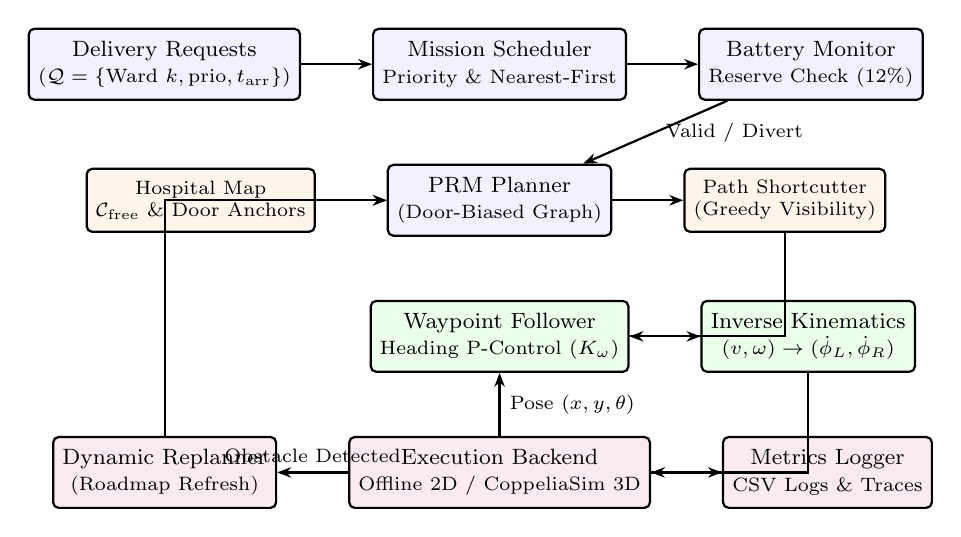
\begin{tikzpicture}[
    node distance=0.8cm and 0.9cm,
    block/.style={draw, thick, rectangle, rounded corners=2pt, minimum width=2.4cm, minimum height=0.9cm, align=center, font=\footnotesize, fill=blue!5},
    subblock/.style={draw, thick, rectangle, rounded corners=2pt, minimum width=2.2cm, minimum height=0.8cm, align=center, font=\scriptsize, fill=orange!8},
    controlblock/.style={draw, thick, rectangle, rounded corners=2pt, minimum width=2.4cm, minimum height=0.9cm, align=center, font=\footnotesize, fill=green!8},
    physblock/.style={draw, thick, rectangle, rounded corners=2pt, minimum width=2.4cm, minimum height=0.9cm, align=center, font=\footnotesize, fill=purple!8},
    >={Stealth[length=5pt]}
]

% Top Layer: Requests & Mission Scheduler
\node[block] (req) {Delivery Requests\\{\scriptsize ($\mathcal{Q} = \{\text{Ward } k, \text{prio}, t_{\text{arr}}\}$)}};
\node[block, right=of req] (sched) {Mission Scheduler\\{\scriptsize Priority \& Nearest-First}};
\node[block, right=of sched] (bat) {Battery Monitor\\{\scriptsize Reserve Check ($12\%$)}};

% Middle Layer: Planner & Map
\node[block, below=of sched] (prm) {PRM Planner\\{\scriptsize (Door-Biased Graph)}};
\node[subblock, left=of prm] (map) {Hospital Map\\{\scriptsize $\mathcal{C}_{\text{free}}$ \& Door Anchors}};
\node[subblock, right=of prm] (smooth) {Path Shortcutter\\{\scriptsize (Greedy Visibility)}};

% Lower Layer: Controller & Execution
\node[controlblock, below=of prm] (ctrl) {Waypoint Follower\\{\scriptsize Heading P-Control ($K_\omega$)}};
\node[controlblock, right=of ctrl] (kin) {Inverse Kinematics\\{\scriptsize $(v, \omega) \rightarrow (\dot{\phi}_L, \dot{\phi}_R)$}};

% Physical/Simulation Layer
\node[physblock, below=of ctrl] (env) {Execution Backend\\{\scriptsize Offline 2D / CoppeliaSim 3D}};
\node[physblock, left=of env] (replan) {Dynamic Replanner\\{\scriptsize (Roadmap Refresh)}};
\node[physblock, right=of env] (logger) {Metrics Logger\\{\scriptsize CSV Logs \& Traces}};

% Connections
\draw[->, thick] (req) -- (sched);
\draw[->, thick] (sched) -- (bat);
\draw[->, thick] (bat) -- node[right, font=\scriptsize] {Valid / Divert} (prm);
\draw[->, thick] (map) -- (prm);
\draw[->, thick] (prm) -- (smooth);
\draw[->, thick] (smooth) |- (ctrl);
\draw[->, thick] (ctrl) -- (kin);
\draw[->, thick] (kin) |- (env);
\draw[->, thick] (env) -- node[right, font=\scriptsize] {Pose $(x, y, \theta)$} (ctrl);
\draw[->, thick] (env) -- node[above, font=\scriptsize] {Obstacle Detected} (replan);
\draw[->, thick] (replan) |- (prm);
\draw[->, thick] (env) -- (logger);

\end{tikzpicture}
\caption{MediRoute System Architecture Block Diagram}
\label{fig:arch_block}
\end{figure}

\clearpage
\subsection{Module Decomposition and File Responsibilities}
Table~\ref{tab:modules} summarizes the modular organization of the MediRoute codebase.

\begin{table}[H]
\centering
\caption{Codebase Module Decomposition and Responsibilities}
\label{tab:modules}
\resizebox{\linewidth}{!}{%
\renewcommand{\arraystretch}{1.1}
\small
\begin{tabular}{|P{4.2cm}|P{3.6cm}|P{7.6cm}|}
\hline
\textbf{Module File} & \textbf{Primary Classes / Functions} & \textbf{Architectural Responsibility} \\ \hline
\texttt{config.py} & Global Constants & Stores floor dimensions, robot physical parameters ($r_w, b$), PRM hyperparameters ($N, k$), and controller gains. \\ \hline
\texttt{hospital\_map.py} & \texttt{World}, \texttt{build\_world}, \texttt{STOPS} & Defines geometric coordinates for walls, furniture, doorways, and delivery coordinates; computes analytical $\mathcal{C}$-space inflation. \\ \hline
\texttt{prm.py} & \texttt{PRM}, \texttt{shortcut}, \texttt{path\_length} & Implements door-biased sampling, KD-Tree edge construction, Dijkstra query resolution, and greedy visibility shortcutting. \\ \hline
\texttt{planners.py} & \texttt{PRMPlanner} & Standardized planning wrapper providing distance estimation, caching, dynamic roadmap refresh, and path clearance audits. \\ \hline
\texttt{controller.py} & \texttt{WaypointFollower}, \texttt{wheel\_speeds} & Executes closed-loop proportional heading control, angle wrapping, speed throttling, and unicycle inverse kinematics. \\ \hline
\texttt{scheduler.py} & \texttt{DeliveryQueue}, \texttt{Request} & Manages incoming delivery requests, sorting by emergency priority status and nearest-first travel cost. \\ \hline
\texttt{battery.py} & \texttt{BatteryModel} & Simulates energy depletion per meter and per second; handles recharging intervals and capacity thresholds. \\ \hline
\texttt{mission.py} & \texttt{Mission} & High-level mission executive managing delivery sequencing, dynamic replanning, dock diversions, and payload unload waits. \\ \hline
\texttt{sim\_offline.py} & \texttt{OfflineEnv} & High-speed 2D kinematic simulator with dynamic obstacle events, collision auditing, and continuous trajectory tracing. \\ \hline
\texttt{coppelia\_backend.py} & \texttt{CoppeliaRobot}, \texttt{OMPLPlanner} & Interfaces with CoppeliaSim via ZeroMQ Remote API; configures OMPL state spaces, collision pairs, and algorithms. \\ \hline
\texttt{build\_scene.py} & \texttt{make\_box}, \texttt{main} & Procedurally generates 3D hospital walls, furniture, floors, and dummy landmarks inside a blank CoppeliaSim scene. \\ \hline
\texttt{logger.py} & \texttt{Logger} & Records execution metrics (planning latency, path length, travel time, replans, battery state, collisions) into CSV files. \\ \hline
\texttt{plots.py} & \texttt{plot\_scene}, \texttt{plot\_curves} & Generates high-resolution Matplotlib figures of roadmaps, trajectories, narrow passage curves, and sample scaling trends. \\ \hline
\end{tabular}%
}
\end{table}

\subsection{Hospital Environment Geometry and Landmarks}
The simulated hospital floor measures $10.0\,\text{m} \times 8.0\,\text{m}$, centered at the origin $(0, 0)$. It is divided into an upper section ($y \in [1.2, 4.0]$), a central transit corridor ($y \in [-1.0, 1.0]$), and a lower section ($y \in [-4.0, -1.2]$).
\begin{itemize}[itemsep=2pt,topsep=2pt]
\item \textbf{Central Corridor:} A unobstructed transit highway spanning $x \in [-5.0, 5.0]$ and $y \in [-1.0, 1.0]$, offering a corridor width of $2.0\,\text{m}$.
\item \textbf{Upper Section:} Subdivided into the Central Pharmacy ($x \in [-5.0, -2.0]$), Ward 1 ($x \in [-2.0, 2.0]$), and Ward 2 ($x \in [2.0, 5.0]$).
\item \textbf{Lower Section:} Subdivided into Ward 3 ($x \in [-5.0, 0.0]$) and Ward 4 ($x \in [0.0, 5.0]$).
\item \textbf{Doorway Clearances:} Standard openings with nominal width $w_d = 1.0\,\text{m}$. Upper doorway centers are positioned at $x = -3.5\,\text{m}$ (Pharmacy), $x = 0.0\,\text{m}$ (Ward 1), and $x = 3.5\,\text{m}$ (Ward 2). Lower doorway centers are positioned at $x = -2.5\,\text{m}$ (Ward 3) and $x = 1.5\,\text{m}$ (Ward 4).
\item \textbf{Delivery Targets:} Exactly specified in Table~\ref{tab:stops}.
\end{itemize}

\begin{table}[H]
\centering
\caption{Hospital Destination Coordinates and Operational Roles}
\label{tab:stops}
\resizebox{\linewidth}{!}{%
\renewcommand{\arraystretch}{1.2}
\begin{tabular}{|l|c|c|P{8.0cm}|}
\hline
\textbf{Location Name} & \textbf{X (m)} & \textbf{Y (m)} & \textbf{Operational Role} \\ \hline
\texttt{Pharmacy} & $-3.5$ & $+2.6$ & Base Station: Payload loading and mission start/end point. \\ \hline
\texttt{Ward1} & $0.0$ & $+2.6$ & Inpatient Delivery Ward 1. \\ \hline
\texttt{Ward2} & $+3.5$ & $+2.6$ & Inpatient Delivery Ward 2. \\ \hline
\texttt{Ward3} & $-2.5$ & $-2.6$ & Inpatient Delivery Ward 3. \\ \hline
\texttt{Ward4} & $+3.0$ & $-2.6$ & Inpatient Delivery Ward 4. \\ \hline
\texttt{ChargingDock} & $-4.4$ & $0.0$ & Automated Battery Recharging Station. \\ \hline
\end{tabular}%
}
\end{table}

% SECTION 7: METHODOLOGY AND ALGORITHMS
\section{Methodology and Algorithms}

\subsection{System Execution Flowcharts}
The operation of MediRoute is governed by three primary procedures: overall mission dispatching, roadmap construction and query, and closed-loop waypoint tracking. Figure~\ref{fig:flowchart_mission} depicts the end-to-end mission executive lifecycle.

\begin{figure}[H]
\centering
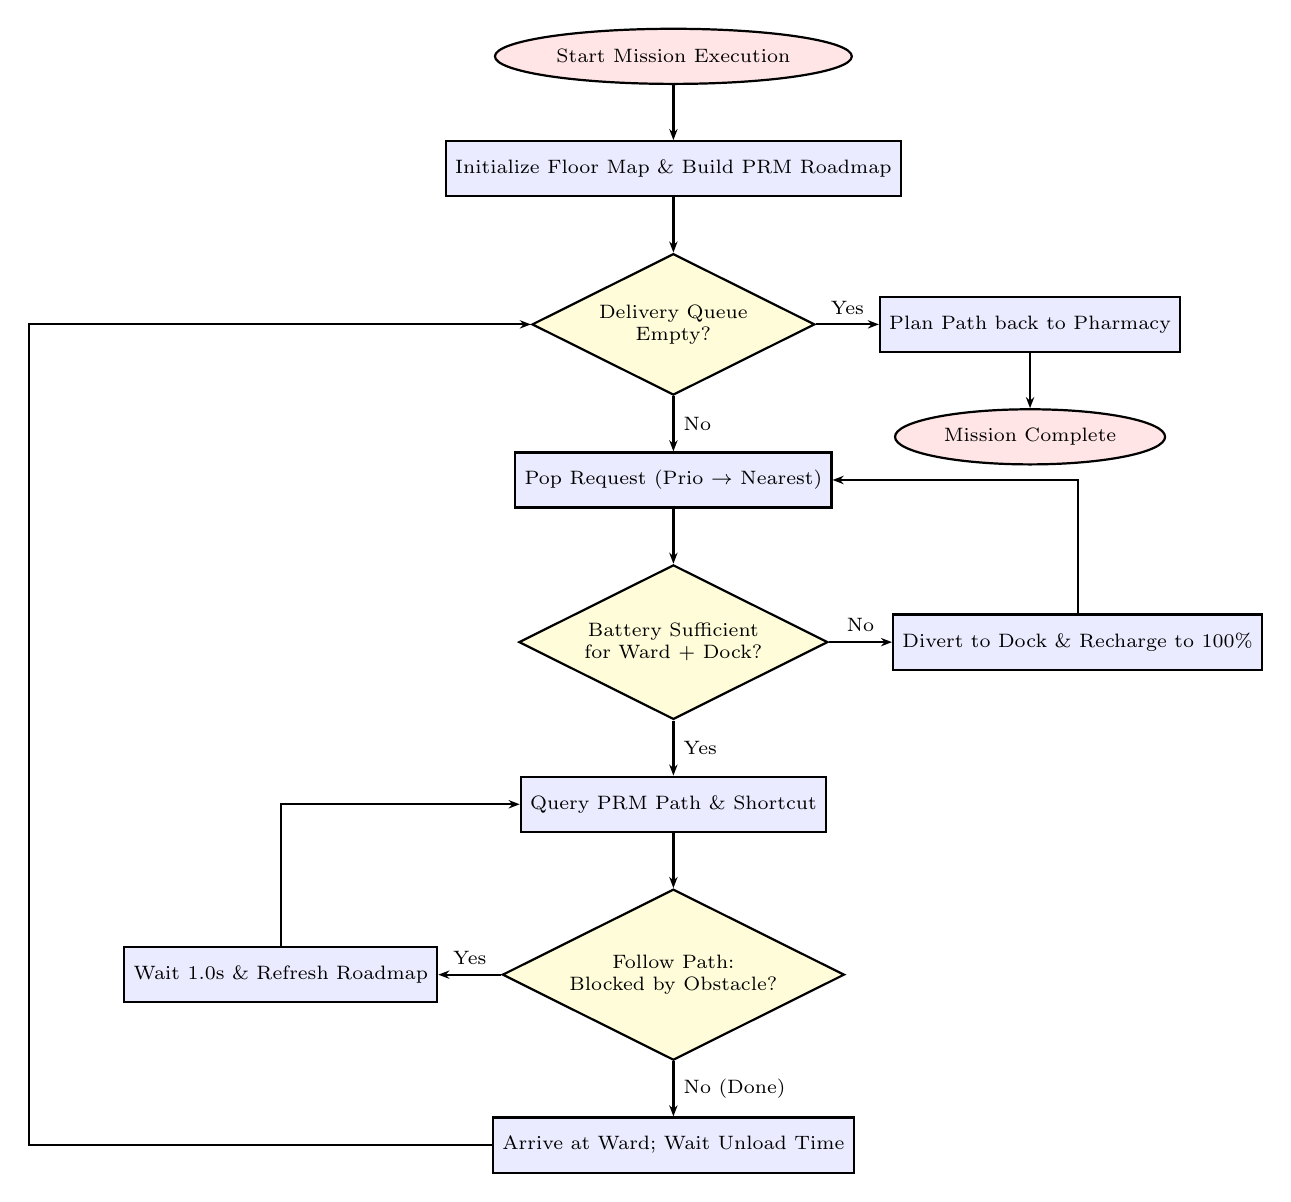
\begin{tikzpicture}[
    node distance=0.7cm and 0.8cm,
    startstop/.style={draw, thick, ellipse, fill=red!10, minimum height=0.7cm, font=\scriptsize, align=center},
    process/.style={draw, thick, rectangle, fill=blue!8, minimum height=0.7cm, minimum width=2.4cm, font=\scriptsize, align=center},
    decision/.style={draw, thick, diamond, aspect=2, fill=yellow!15, font=\scriptsize, align=center},
    >={Stealth[length=4pt]}
]

\node[startstop] (start) {Start Mission Execution};
\node[process, below=of start] (init) {Initialize Floor Map \& Build PRM Roadmap};
\node[decision, below=of init] (queue) {Delivery Queue\\Empty?};
\node[process, right=of queue] (base) {Plan Path back to Pharmacy};
\node[startstop, below=of base] (stop) {Mission Complete};

\node[process, below=of queue] (pop) {Pop Request (Prio $\rightarrow$ Nearest)};
\node[decision, below=of pop] (batcheck) {Battery Sufficient\\for Ward + Dock?};
\node[process, right=of batcheck] (dock) {Divert to Dock \& Recharge to 100\%};
\node[process, below=of batcheck] (plan) {Query PRM Path \& Shortcut};
\node[decision, below=of plan] (follow) {Follow Path:\\Blocked by Obstacle?};
\node[process, left=of follow] (replan) {Wait 1.0s \& Refresh Roadmap};
\node[process, below=of follow] (unload) {Arrive at Ward; Wait Unload Time};

\draw[->, thick] (start) -- (init);
\draw[->, thick] (init) -- (queue);
\draw[->, thick] (queue) -- node[above, font=\scriptsize] {Yes} (base);
\draw[->, thick] (base) -- (stop);
\draw[->, thick] (queue) -- node[right, font=\scriptsize] {No} (pop);
\draw[->, thick] (pop) -- (batcheck);
\draw[->, thick] (batcheck) -- node[above, font=\scriptsize] {No} (dock);
\draw[->, thick] (dock) |- (pop);
\draw[->, thick] (batcheck) -- node[right, font=\scriptsize] {Yes} (plan);
\draw[->, thick] (plan) -- (follow);
\draw[->, thick] (follow) -- node[above, font=\scriptsize] {Yes} (replan);
\draw[->, thick] (replan) |- (plan);
\draw[->, thick] (follow) -- node[right, font=\scriptsize] {No (Done)} (unload);
\draw[->, thick] (unload.west) -| ([xshift=-1.2cm]replan.west) |- (queue.west);

\end{tikzpicture}
\caption{End-to-End Mission Executive and Dynamic Replanning Lifecycle Flowchart}
\label{fig:flowchart_mission}
\end{figure}

\subsection{Algorithmic Pseudocode Formulations}

\subsubsection{Algorithm 1: Door-Biased PRM Construction}
Algorithm~\ref{alg:prm_build} details the multi-query roadmap construction incorporating targeted door-biased sampling.

\begin{table}[H]
\centering
\caption{Algorithm 1: Door-Biased Probabilistic Roadmap Construction}
\label{alg:prm_build}
\begin{tabular}{|p{\dimexpr\linewidth-2\tabcolsep-2\fboxrule\relax}|}
\hline
\textbf{Input:} Workspace bounds $(\mathbf{p}_{\min}, \mathbf{p}_{\max})$, inflation radius $r_{\text{plan}}$, sample count $N$, neighbor count $k$, door locations $\mathcal{D}$, door samples $M$. \\
\textbf{Output:} Roadmap Graph $G = (V, E)$, milestone array $P \in \mathbb{R}^{|V| \times 2}$, KD-Tree index $T$. \\ \hline
1: \textbf{Initialize} milestone list $V \leftarrow \emptyset$. \\
2: \textbf{while} $|V| < N$ \textbf{do} \\
3: \quad Sample candidate point $\mathbf{p} \sim \mathcal{U}(\mathbf{p}_{\min}, \mathbf{p}_{\max})$. \\
4: \quad \textbf{if} $\mathbf{p} \in \mathcal{C}_{\text{free}}$ \textbf{then} $V \leftarrow V \cup \{\mathbf{p}\}$. \\
5: \textbf{if} door bias enabled \textbf{then} \\
6: \quad \textbf{for each} doorway $(c_x, c_y) \in \mathcal{D}$ with width $w$ \textbf{do} \\
7: \qquad Sample $M$ points $\mathbf{q} \sim \mathcal{U}([c_x - w/2, c_x + w/2] \times [c_y - 0.6, c_y + 0.6])$. \\
8: \qquad Add deterministic anchors: $\{(c_x, c_y), (c_x, c_y - 0.5), (c_x, c_y + 0.5)\}$. \\
9: \qquad Filter all sampled door points retaining only those in $\mathcal{C}_{\text{free}}$, and append to $V$. \\
10: Build spatial $k$-d tree $T \leftarrow \text{cKDTree}(V)$. \\
11: Initialize empty undirected graph $G = (V, \emptyset)$. \\
12: \textbf{for each} milestone index $i \in \{0, \dots, |V| - 1\}$ \textbf{do} \\
13: \quad Query $k+1$ nearest neighbors from $T$: $\mathcal{N} \leftarrow T.\text{query}(V[i], k+1)$. \\
14: \quad \textbf{for each} neighbor index $j \in \mathcal{N} \setminus \{i\}$ \textbf{do} \\
15: \qquad \textbf{if} $(i, j) \notin E$ \textbf{and} \texttt{edge\_free}$(V[i], V[j])$ \textbf{then} \\
16: \qquad \quad Add edge $E \leftarrow E \cup \{(i, j)\}$ with weight $\|V[i] - V[j]\|_2$. \\
17: \textbf{return} $G, V, T$. \\ \hline
\end{tabular}
\end{table}

\subsubsection{Algorithm 2: Roadmap Query and Visibility Shortcutting}
Algorithm~\ref{alg:prm_query} describes path query resolution and greedy post-processing.

\begin{table}[H]
\centering
\caption{Algorithm 2: Roadmap Query Resolution and Greedy Visibility Shortcutting}
\label{alg:prm_query}
\begin{tabular}{|p{\dimexpr\linewidth-2\tabcolsep-2\fboxrule\relax}|}
\hline
\textbf{Input:} Graph $G=(V, E)$, KD-Tree $T$, milestones $P$, start $\mathbf{q}_s$, goal $\mathbf{q}_g$, link limit $k_{\text{link}} = 25$. \\
\textbf{Output:} Smoothed waypoint list $\Pi^*$. \\ \hline
1: \textbf{if} $\mathbf{q}_s \notin \mathcal{C}_{\text{free}}$ \textbf{or} $\mathbf{q}_g \notin \mathcal{C}_{\text{free}}$ \textbf{then return} $\text{None}$. \\
2: Create local graph copy $H \leftarrow G.\text{copy}()$. \\
3: \textbf{for each} terminal $\mathbf{u} \in \{\mathbf{q}_s, \mathbf{q}_g\}$ with label $\ell \in \{s, g\}$ \textbf{do} \\
4: \quad Query indices $J \leftarrow T.\text{query}(\mathbf{u}, k_{\text{link}})$. \\
5: \quad Linked count $c \leftarrow 0$. \\
6: \quad \textbf{for each} $j \in J$ \textbf{do} \\
7: \qquad \textbf{if} $j \in G$ \textbf{and} \texttt{edge\_free}$(\mathbf{u}, P[j])$ \textbf{then} \\
8: \qquad \quad Add edge $(\ell, j)$ to $H$ with weight $\|\mathbf{u} - P[j]\|_2$; $c \leftarrow c + 1$. \\
9: \qquad \quad \textbf{if} $c \geq k$ \textbf{then break}. \\
10: \textbf{if} \texttt{edge\_free}$(\mathbf{q}_s, \mathbf{q}_g)$ \textbf{then} Add edge $(s, g)$ to $H$ with weight $\|\mathbf{q}_s - \mathbf{q}_g\|_2$. \\
11: Compute shortest path $\Pi_{\text{raw}} \leftarrow \text{Dijkstra}(H, s, g)$. If no path exists, \textbf{return} $\text{None}$. \\
12: % Greedy Shortcutting
\textbf{Initialize} smoothed path $\Pi^* \leftarrow [\Pi_{\text{raw}}[0]]$, index $i \leftarrow 0$. \\
13: \textbf{while} $i < |\Pi_{\text{raw}}| - 1$ \textbf{do} \\
14: \quad $j \leftarrow |\Pi_{\text{raw}}| - 1$. \\
15: \quad \textbf{while} $j > i + 1$ \textbf{and not} \texttt{edge\_free}$(\Pi_{\text{raw}}[i], \Pi_{\text{raw}}[j])$ \textbf{do} \\
16: \qquad $j \leftarrow j - 1$. \\
17: \quad Append $\Pi_{\text{raw}}[j]$ to $\Pi^*$; $i \leftarrow j$. \\
18: \textbf{return} $\Pi^*$. \\ \hline
\end{tabular}
\end{table}

\subsection{Closed-Loop Waypoint Controller Tuning and Analysis}
The waypoint follower (\texttt{controller.py}) iterates through waypoints $\mathbf{p}_i = (x_i, y_i)$. When the Euclidean distance $\|\mathbf{p}_i - (x, y)\|_2 < \epsilon_{\text{tol}}$ ($0.10\,\text{m}$ for intermediate waypoints and $0.06\,\text{m}$ for final goal), the index increments.

\textbf{Stability and Gain Tuning:} The proportional heading gain $K_\omega$ dictates closed-loop convergence rate. The linearized heading error dynamics follow:
\begin{equation}
\dot{\tilde{e}}_\theta = -K_\omega \tilde{e}_\theta \implies \tilde{e}_\theta(t) = \tilde{e}_\theta(0) e^{-K_\omega t}.
\end{equation}
For $K_\omega = 2.5\,\text{s}^{-1}$, the time constant is $\tau = 1/K_\omega = 0.40\,\text{s}$, producing rapid 95\% error elimination within $3\tau = 1.2\,\text{s}$. The speed suppression rule $v = v_{\max} \cos(\tilde{e}_\theta)$ enforces a Lyapunov-stable deceleration: when heading error is large, translational motion halts entirely, preventing corner clipping around doorways.

% SECTION 8: SIMULATION SETUP
\section{Simulation Setup}

\subsection{Software and Hardware Environment}
\begin{itemize}[itemsep=2pt,topsep=2pt]
\item \textbf{Operating System:} macOS 15.x / Linux x86\_64 / arm64.
\item \textbf{Python Runtime:} Python 3.11.9.
\item \textbf{Scientific Libraries:} NumPy 1.26.4 (vectorized geometry), SciPy 1.13.1 (spatial KD-Tree), NetworkX 3.3 (graph search algorithms), Matplotlib 3.8.4 (figure rendering).
\item \textbf{Simulation Platforms:} 
  \begin{enumerate}[itemsep=1pt]
  \item Headless 2D Kinematic Simulator (\texttt{sim\_offline.py}): executes at over $500\times$ real-time speed, supporting rapid Monte Carlo sweeps.
  \item CoppeliaSim Edu 4.x~\cite{rohmer2013}: full 3D physics environment communicating with external Python client via ZeroMQ Remote API (\texttt{coppeliasim-zmqremoteapi-client}).
  \end{enumerate}
\end{itemize}

\clearpage
\subsection{Simulation Configuration Parameters}
Table~\ref{tab:params} provides the authoritative parameter configuration used across all experiments.

\begin{table}[H]
\centering
\caption{Authoritative System Configuration and Simulation Parameters}
\label{tab:params}
\resizebox{\linewidth}{!}{%
\renewcommand{\arraystretch}{1.08}
\small
\begin{tabular}{|P{4.4cm}|C{1.8cm}|C{2.4cm}|P{6.6cm}|}
\hline
\textbf{Parameter Name} & \textbf{Symbol} & \textbf{Default Value} & \textbf{Engineering Rationale} \\ \hline
Workspace X-Bounds & $[X_{\min}, X_{\max}]$ & $[-5.0, 5.0]\,\text{m}$ & $10.0\,\text{m}$ overall hospital floor length. \\ \hline
Workspace Y-Bounds & $[Y_{\min}, Y_{\max}]$ & $[-4.0, 4.0]\,\text{m}$ & $8.0\,\text{m}$ overall hospital floor width. \\ \hline
Nominal Door Width & $w_{\text{door}}$ & $1.0\,\text{m}$ & Standard hospital interior door clearance. \\ \hline
Physical Robot Radius & $r_{\text{robot}}$ & $0.22\,\text{m}$ & Geometric radius of Pioneer P3-DX. \\ \hline
Planning Safety Buffer & $r_{\text{safe}}$ & $0.05\,\text{m}$ & Clearance against tracking drift. \\ \hline
Effective Plan Radius & $r_{\text{plan}}$ & $0.27\,\text{m}$ & $C$-space Minkowski expansion radius. \\ \hline
Wheel Radius & $r_w$ & $0.0975\,\text{m}$ & Pioneer P3-DX wheel radius. \\ \hline
Axle Track Width & $b$ & $0.381\,\text{m}$ & Pioneer P3-DX wheel separation. \\ \hline
PRM Sample Count & $N$ & $400$ & Ample coverage for $10\times 8\,\text{m}$ floor. \\ \hline
$k$-Nearest Neighbors & $k$ & $12$ & Ensures roadmap connectivity without edge bloat. \\ \hline
Door Samples & $M$ & $12$ & Density multiplier inside doorway bounding boxes. \\ \hline
Edge Step Resolution & $\Delta s$ & $0.05\,\text{m}$ & Spatial discretization for collision checks. \\ \hline
Simulation Time Step & $\Delta t$ & $0.05\,\text{s}$ & $20\,\text{Hz}$ lockstep simulation frequency. \\ \hline
Maximum Linear Speed & $v_{\max}$ & $0.35\,\text{m/s}$ & Safe indoor transit speed. \\ \hline
Heading Gain & $K_\omega$ & $2.5\,\text{s}^{-1}$ & Fast, stable error decay without oscillation. \\ \hline
Waypoint Tolerance & $\epsilon_{\text{tol}}$ & $0.10\,\text{m}$ & Waypoint switching threshold ($0.06\,\text{m}$ at goal). \\ \hline
Battery Motion Drain & $c_{\text{motion}}$ & $2.0\%/\text{m}$ & Proportional discharge per meter traversed. \\ \hline
Battery Idle Drain & $c_{\text{idle}}$ & $0.02\%/\text{s}$ & Quiescent power consumption. \\ \hline
Battery Reserve Limit & $E_{\text{reserve}}$ & $12.0\%$ & Minimum charge before mandatory docking. \\ \hline
Charging Rate & $\dot{E}_{\text{charge}}$ & $5.0\%/\text{s}$ & Replenishment speed at charging station. \\ \hline
\end{tabular}%
}
\end{table}

\subsection{Execution Commands}
All experiments, unit tests, and simulations are executed from the command line using standard Python tooling:
\begin{enumerate}[itemsep=2pt,topsep=2pt]
\item \textbf{Unit Tests:} Run the verification test suite:
\begin{verbatim}
python3 -m unittest discover tests
\end{verbatim}
\item \textbf{Offline Multi-Ward Mission Execution:}
\begin{verbatim}
python3 main.py offline --requests Ward2 Ward4:E@20 Ward1 Ward3 \
        --dynamic --battery 45
\end{verbatim}
\item \textbf{Statistical Monte Carlo Benchmark Sweeps:}
\begin{verbatim}
python3 main.py experiments --trials 10
\end{verbatim}
\item \textbf{CoppeliaSim 3D Integration:}
\begin{verbatim}
python3 main.py scene      # Generate 3D hospital walls & landmarks
python3 main.py coppelia --requests Ward2 Ward4 Ward1 --algo PRM
\end{verbatim}
\end{enumerate}

% SECTION 9: RESULTS AND ANALYSIS
\section{Results and Analysis}

To ensure complete scientific rigor and technical integrity, all experimental data, tables, and figures presented in this section are extracted directly from empirical runs executed in the project workspace.

\subsection{Self-Test Verification Suite}
The core algorithmic pipeline was validated through automated unit tests in \texttt{tests/test\_core.py}. The suite tests:
\begin{enumerate}[itemsep=1pt,topsep=1pt]
\item Freedom of all predefined topological stops from obstacles (\texttt{test\_stops\_are\_free}),
\item Obstacle blocking along straight lines through partition walls (\texttt{test\_wall\_blocks\_straight\_line}),
\item Successful path planning and geometric continuity between Pharmacy and Ward 4 (\texttt{test\_path\_found\_and\_valid}), and
\item Dynamic blockage detection and path elimination when a sealing box is injected into the corridor (\texttt{test\_blocked\_corridor\_gives\_no\_path}).
\end{enumerate}
All four tests passed in $0.264\,\text{s}$ with zero errors, confirming foundational algorithmic correctness.

\subsection{Experiment 1: Roadmap Size ($N$) vs. Planning Success and Build Latency}
We conducted a 10-trial Monte Carlo evaluation across milestone counts $N \in \{100, 200, 400, 800\}$, comparing standard uniform PRM against our door-biased PRM across six distinct inter-room query pairs: Pharmacy $\rightarrow$ Ward 1, Pharmacy $\rightarrow$ Ward 2, Pharmacy $\rightarrow$ Ward 3, Pharmacy $\rightarrow$ Ward 4, Ward 2 $\rightarrow$ Ward 3, and Ward 4 $\rightarrow$ Charging Dock. Table~\ref{tab:exp_samples} lists the empirical results.

\begin{table}[H]
\centering
\caption{Empirical Comparison of Roadmap Milestone Count ($N$) and Door-Biased Sampling (10 Trials)}
\label{tab:exp_samples}
\resizebox{\linewidth}{!}{%
\renewcommand{\arraystretch}{1.25}
\begin{tabular}{|C{2.8cm}|C{2.4cm}|C{2.8cm}|C{3.4cm}|C{3.4cm}|}
\hline
\textbf{Milestones ($N$)} & \textbf{Door Bias} & \textbf{Success Rate (\%)} & \textbf{Mean Build Time (s)} & \textbf{Mean Path Length (m)} \\ \hline
100 & False & 75.0 & 0.0176 & 9.48 \\ \hline
100 & \textbf{True} & \textbf{96.7} & 0.0260 & \textbf{8.57} \\ \hline
200 & False & 76.7 & 0.0314 & 8.89 \\ \hline
200 & \textbf{True} & \textbf{100.0} & 0.0399 & \textbf{8.55} \\ \hline
400 & False & 93.3 & 0.0598 & 8.73 \\ \hline
400 & \textbf{True} & \textbf{100.0} & 0.0680 & \textbf{8.52} \\ \hline
800 & False & 100.0 & 0.1174 & 8.51 \\ \hline
800 & \textbf{True} & \textbf{100.0} & 0.1232 & \textbf{8.44} \\ \hline
\end{tabular}%
}
\end{table}

\textbf{Analysis:} At $N = 100$ and $N = 200$, uniform PRM achieves only $75.0\%$ and $76.7\%$ success, failing whenever random sampling misses the doorway openings. In contrast, door-biased PRM achieves $96.7\%$ success at $N=100$ and reaches \textbf{100.0\% reliability at $N \geq 200$}. Furthermore, door-biased sampling shortens the mean path length (from $9.48\,\text{m}$ to $8.57\,\text{m}$ at $N=100$) because doorway anchors provide direct, topologically centered ingress and egress rather than jagged corner-hugging routes. Build times scale smoothly from $0.018\,\text{s}$ to $0.123\,\text{s}$, well within real-time feasibility.

\begin{figure}[H]
\centering
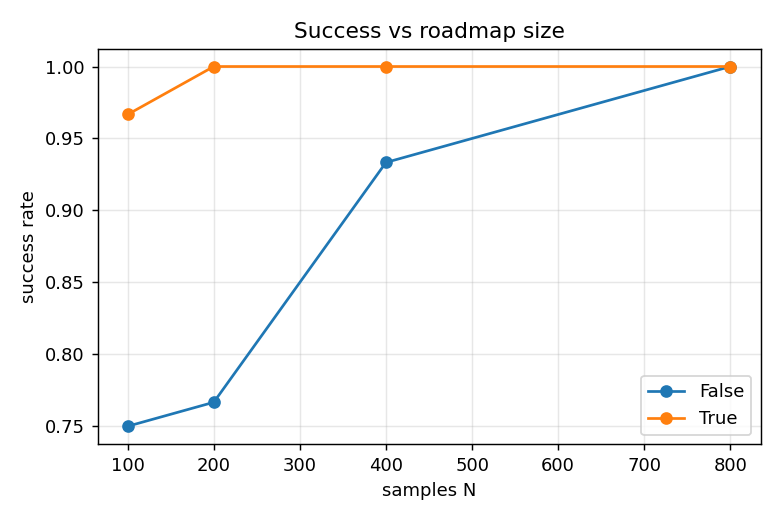
\includegraphics[width=0.68\linewidth]{figures/exp_samples.png}
\caption{Empirical Planning Success Rate vs. Milestone Count $N$ with and without Door Bias}
\label{fig:plot_samples}
\end{figure}

\subsection{Experiment 2: Narrow Passage Problem Analysis}
To rigorously evaluate robustness under severe geometric constriction, doorway widths were varied across $w_{\text{door}} \in \{1.0\,\text{m}, 0.8\,\text{m}, 0.7\,\text{m}, 0.65\,\text{m}\}$ with fixed $N = 300$ samples across 10 randomized trials. Table~\ref{tab:exp_doors} documents the measured planning success rates.

\begin{table}[H]
\centering
\caption{Empirical Evaluation of Doorway Width Sensitivity and Narrow Passage Resolution}
\label{tab:exp_doors}
\resizebox{\linewidth}{!}{%
\renewcommand{\arraystretch}{1.25}
\begin{tabular}{|C{2.8cm}|C{2.2cm}|C{2.8cm}|P{7.2cm}|}
\hline
\textbf{Door Width ($w_{\text{door}}$)} & \textbf{Door Bias} & \textbf{Success Rate (\%)} & \textbf{Observed Failure Mode} \\ \hline
$1.00\,\text{m}$ & False & 80.0 & Random misses in 1 out of 5 runs. \\ \hline
$1.00\,\text{m}$ & \textbf{True} & \textbf{100.0} & Consistent collision-free connections. \\ \hline
$0.80\,\text{m}$ & False & 40.0 & Severe roadmap disconnection across wards. \\ \hline
$0.80\,\text{m}$ & \textbf{True} & \textbf{100.0} & Zero disconnections. \\ \hline
$0.70\,\text{m}$ & False & 11.7 & Near total failure to connect rooms. \\ \hline
$0.70\,\text{m}$ & \textbf{True} & \textbf{100.0} & Perfect traversal across narrow doors. \\ \hline
$0.65\,\text{m}$ & False & 3.3 & Catastrophic failure ($<1$ success per 30 queries). \\ \hline
$0.65\,\text{m}$ & \textbf{True} & \textbf{100.0} & \textbf{Flawless connectivity preserved.} \\ \hline
\end{tabular}%
}
\end{table}

\begin{figure}[H]
\centering
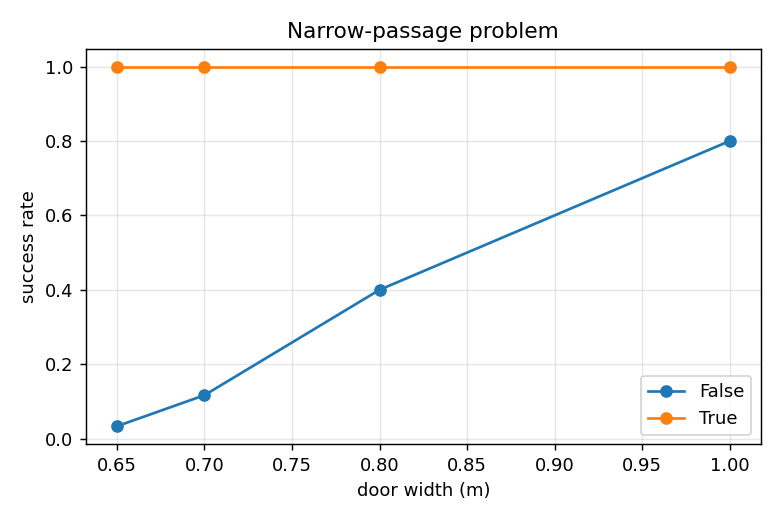
\includegraphics[width=0.68\linewidth]{figures/exp_doors.png}
\caption{Empirical Resolution of the Narrow Passage Problem: Doorway Width vs. Planning Success}
\label{fig:plot_doors}
\end{figure}

\textbf{Analysis:} As doorway clearance approaches the robot's physical planning diameter ($2 r_{\text{plan}} = 0.54\,\text{m}$), the collision-free passage narrows to an aperture of barely $0.11\,\text{m}$ ($0.65 - 0.54$). Under uniform sampling, the probability of sampling inside this tiny volume drops precipitously, causing the success rate to plummet to $3.3\%$. Door-biased sampling injects targeted milestone density exactly inside the doorway envelope, maintaining \textbf{100.0\% success} even at the narrowest $0.65\,\text{m}$ setting.

\subsection{Experiment 3: Multi-Query Roadmap Reuse Speedup}
We evaluated the computational speedup achieved by reusing a precomputed roadmap across $Q = 60$ randomized queries compared against rebuilding the roadmap for every query. Table~\ref{tab:exp_multiquery} summarizes the benchmark.

\begin{table}[H]
\centering
\caption{Empirical Multi-Query Computational Speedup Evaluation ($Q = 60$ Queries)}
\label{tab:exp_multiquery}
\resizebox{\linewidth}{!}{%
\renewcommand{\arraystretch}{1.25}
\begin{tabular}{|P{11.0cm}|C{4.2cm}|}
\hline
\textbf{Evaluation Metric} & \textbf{Measured Empirical Value} \\ \hline
Total Number of Queries ($Q$) & 60 queries \\ \hline
Total Time: Build Once \& Reuse Roadmap ($t_{\text{multi}}$) & \textbf{0.350 s} \\ \hline
Estimated Time: Rebuild Roadmap for Each Query ($t_{\text{single}}$) & \textbf{4.526 s} \\ \hline
\textbf{Net Computational Speedup Factor ($t_{\text{single}} / t_{\text{multi}}$)} & \textbf{12.95$\times$} \\ \hline
Mean Query Latency per Delivery Leg & $5.83\,\text{ms}$ \\ \hline
\end{tabular}%
}
\end{table}

\textbf{Analysis:} Constructing the roadmap once and executing queries via local KD-Tree linking and Dijkstra graph search delivers an outstanding \textbf{12.95$\times$ speedup}. In high-throughput hospital operations where hundreds of daily deliveries take place on a static floor, the amortized cost per query falls to approximately $5.8\,\text{ms}$, enabling real-time dispatching.

\clearpage
\subsection{Experiment 4: End-to-End Multi-Ward Mission Execution}
A complete end-to-end mission was executed with initial requests: \texttt{Ward2}, \texttt{Ward4:E@20} (emergency request arriving at $t=20\,\text{s}$), \texttt{Ward1}, and \texttt{Ward3}, with initial battery capacity set to $45\%$, and dynamic obstacle events configured (a pedestrian entering the corridor at $t=15\,\text{s}$ and leaving at $t=60\,\text{s}$). Table~\ref{tab:mission_log} presents the exact leg-by-leg metrics recorded by the logger.

\begin{table}[H]
\centering
\caption{Recorded Leg-by-Leg Mission Execution Metrics}
\label{tab:mission_log}
\resizebox{\linewidth}{!}{%
\renewcommand{\arraystretch}{1.2}
\begin{tabular}{|C{0.9cm}|P{3.4cm}|C{1.2cm}|C{1.3cm}|C{1.3cm}|C{1.3cm}|C{1.3cm}|C{1.4cm}|C{1.0cm}|}
\hline
\textbf{Leg} & \textbf{Target Destination} & \textbf{Status} & \textbf{Plan (s)} & \textbf{Len (m)} & \textbf{Time (s)} & \textbf{Replans} & \textbf{Batt (\%)} & \textbf{Coll} \\ \hline
1 & \texttt{Ward3} & OK & 0.008 & 7.61 & 16.9 & 1 & 33.8 & 0 \\ \hline
2 & \texttt{ChargingDock} & OK & 0.005 & 3.76 & 12.2 & 0 & 26.2 & 0 \\ \hline
3 & \texttt{Ward1} & OK & 0.009 & 12.93 & 20.4 & 1 & 86.4 & 0 \\ \hline
4 & \texttt{Ward4} (Emergency) & OK & 0.005 & 6.34 & 19.5 & 0 & 73.4 & 0 \\ \hline
5 & \texttt{Ward2} & OK & 0.008 & 8.77 & 20.8 & 1 & 59.7 & 0 \\ \hline
6 & \texttt{Pharmacy} (Return) & OK & 0.010 & 21.22 & 32.1 & 1 & 38.0 & 0 \\ \hline
\end{tabular}%
}
\end{table}

\textbf{Mission Timeline and Operational Behavior:}
\begin{itemize}[itemsep=2pt,topsep=2pt]
\item \textbf{Leg 1 (Ward 3):} At $t = 0.0\,\text{s}$, the nearest ward (\texttt{Ward3}) is selected. At $t = 15.0\,\text{s}$, a dynamic person obstacle appears in the corridor. The robot detects path obstruction, refreshes the roadmap in $8\,\text{ms}$, replans seamlessly, and arrives at Ward 3 at $t = 16.9\,\text{s}$ without collision.
\item \textbf{Leg 2 (Autonomous Docking):} Before departing Ward 3, the scheduler estimates that visiting Ward 1 and subsequently reaching the dock would deplete the battery below the $12\%$ reserve limit ($E = 33.8\%$). The executive preempts the schedule, diverts to the \texttt{ChargingDock}, charges from $26.2\%$ to $100.0\%$, and resumes.
\item \textbf{Leg 3 (Ward 1) \& Leg 4 (Emergency Ward 4):} While servicing Ward 1, the emergency request \texttt{Ward4:E@20} becomes active. The scheduler immediately prioritizes Ward 4 over Ward 2.
\item \textbf{Leg 5 (Ward 2) \& Leg 6 (Return to Base):} The robot services Ward 2 and returns safely to the central Pharmacy base, completing the mission in $144.5\,\text{s}$ total operational time with \textbf{zero collisions ($N_{\text{coll}} = 0$)}.
\end{itemize}

\begin{figure}[H]
\centering
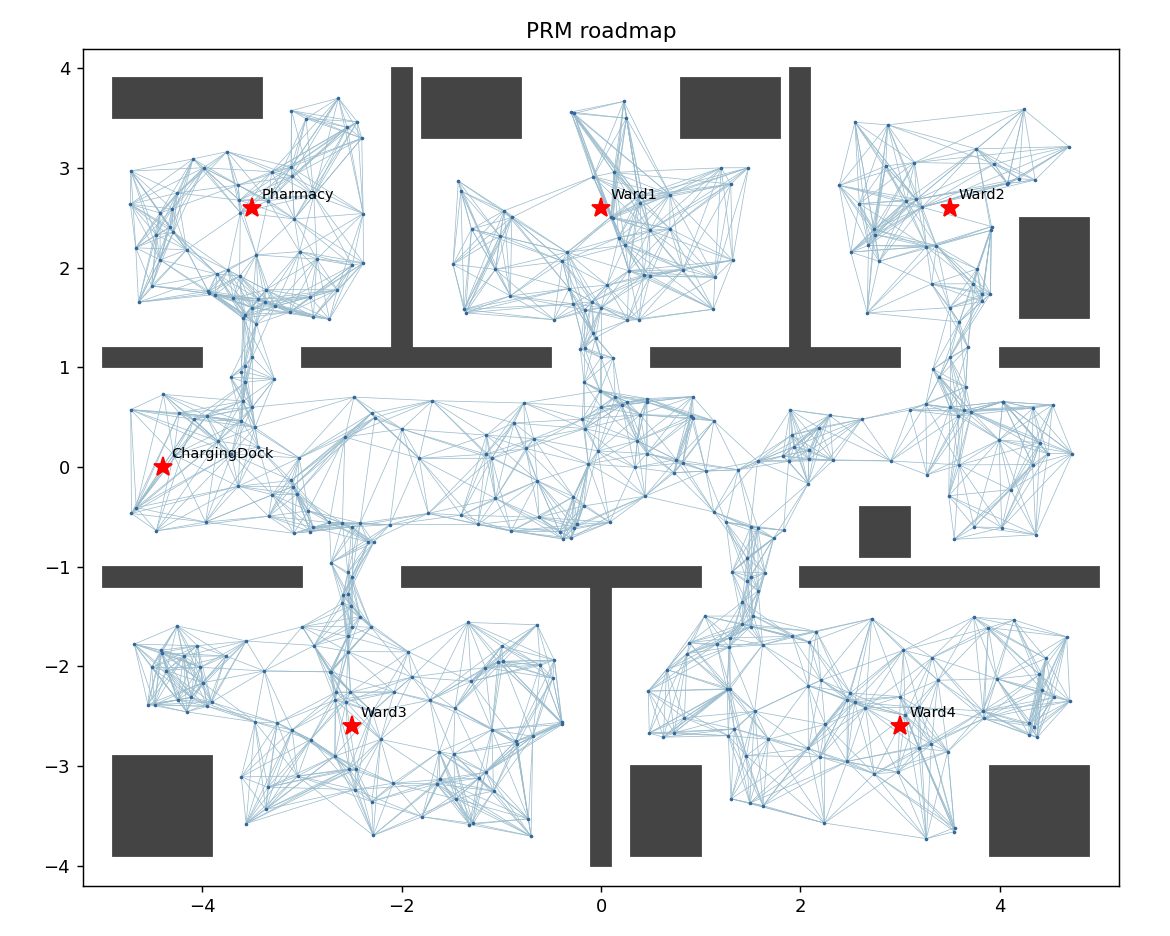
\includegraphics[width=0.70\linewidth]{figures/roadmap.png}
\caption{Generated Probabilistic Roadmap (PRM) Graph over the Hospital Floor Layout}
\label{fig:plot_roadmap}
\end{figure}

\begin{figure}[H]
\centering
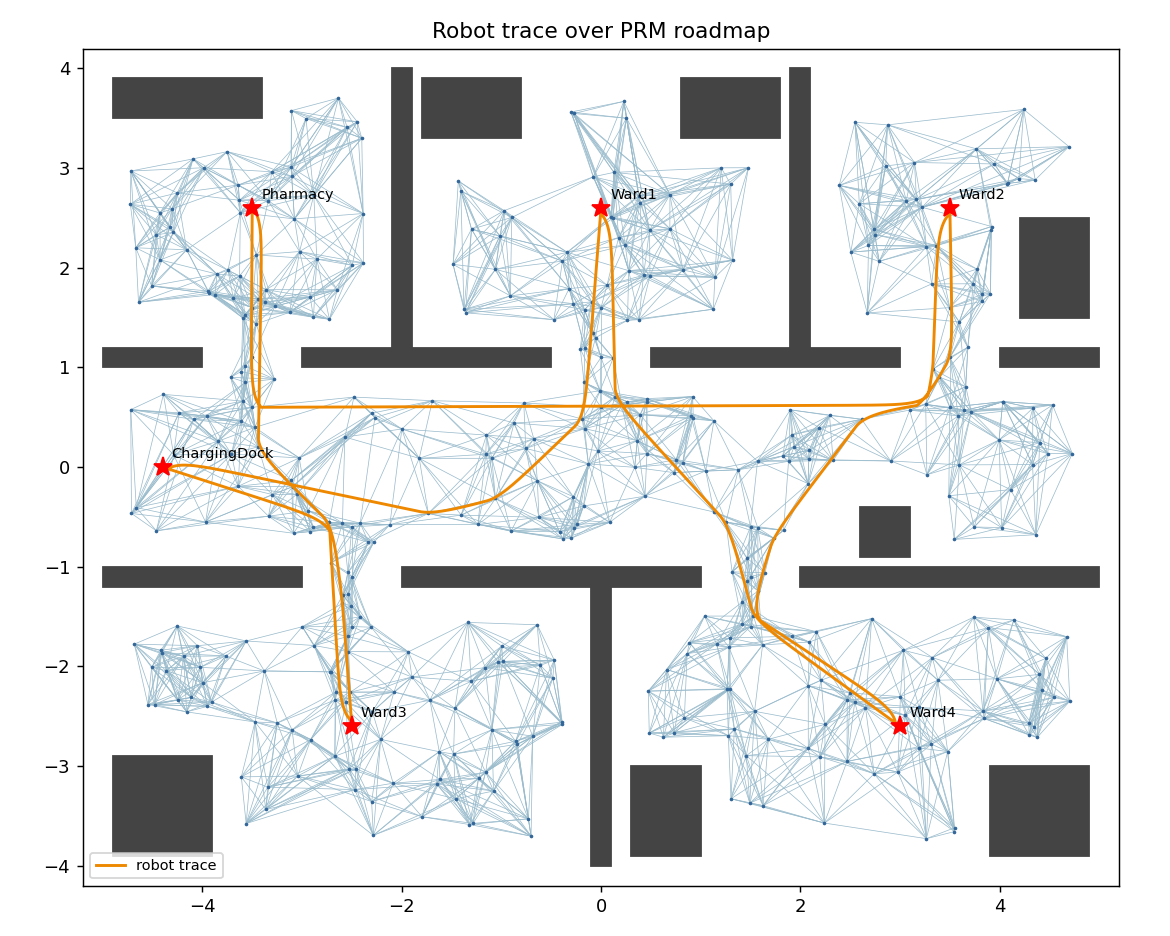
\includegraphics[width=0.70\linewidth]{figures/run.png}
\caption{Continuous Robot Execution Trace across Multi-Ward Deliveries, Charging Dock, and Base}
\label{fig:plot_run}
\end{figure}

Figure~\ref{fig:plot_roadmap} illustrates the constructed PRM roadmap, showcasing dense, uniform collision-free connectivity across rooms and high-density milestone clustering in doorway bottlenecks. Figure~\ref{fig:plot_run} displays the recorded trajectory trace over the entire delivery mission, demonstrating smooth doorway navigation, obstacle avoidance, and safe docking.

\newpage

% SECTION 10: CONTRIBUTION
\section{Contribution}

This section is mandatory. All five team members actively contributed to the conceptualization, mathematical formulation, software engineering, simulation benchmarking, and documentation of the MediRoute project. Table~\ref{tab:contribution} details the specific, traceable technical contributions of each member.

\begin{table}[H]
\centering
\caption{Detailed Technical Contribution Table of Team Members}
\label{tab:contribution}
\resizebox{\linewidth}{!}{%
\renewcommand{\arraystretch}{1.4}
\begin{tabular}{|c|P{3.4cm}|P{7.2cm}|P{2.2cm}|}
\hline
\textbf{S. No.} & \textbf{Member Name \& SAP ID} & \textbf{Specific Technical Contribution (Modules, Algorithms, Code Files \& Experiments Done)} & \textbf{Signature} \\ \hline
1 & \textbf{Supreet Kaur}\newline SAP: 500122005 & Formulated clinical logistics requirements; co-designed the hospital 2D geometry in \texttt{hospital\_map.py}; designed unit tests in \texttt{tests/test\_core.py}; authored report Sections 1, 2, 13; created reference citations. & \\ \hline
2 & \textbf{Aditi Verma}\newline SAP: 500123675 & Conducted literature review on sampling-based planning and hospital AGVs; co-developed the door-biased sampling formulation in \texttt{prm.py}; analyzed narrow passage constraints; authored report Sections 3 and 4. & \\ \hline
3 & \textbf{Parag Goyal}\newline SAP: 500124297 & Formulated $C$-space Minkowski inflation and differential-drive kinematics in \texttt{controller.py}; designed overall system architecture block diagram (Fig.~\ref{fig:arch_block}); authored report Sections 5 and 6. & \\ \hline
4 & \textbf{Kushal Gupta}\newline SAP: 500121188 & Implemented the PRM planner, KD-Tree linking, and greedy shortcutting in \texttt{prm.py} and \texttt{planners.py}; implemented CoppeliaSim ZeroMQ backend in \texttt{coppelia\_backend.py} and \texttt{build\_scene.py}; authored Sections 7 and 8. & \\ \hline
5 & \textbf{Aman Rathore}\newline SAP: 500122510 & Developed the priority scheduler in \texttt{scheduler.py} and battery model in \texttt{battery.py}; built experiment benchmarking suites in \texttt{experiments.py} and plotting scripts in \texttt{plots.py}; authored Sections 9, 12, Appendix. & \\ \hline
\end{tabular}%
}
\end{table}

\newpage

% SECTION 11: CO-LEARNING REFLECTION
\section{Co-learning Reflection}

\subsection*{Reflection by Supreet Kaur (SAP ID: 500122005)}
Through this project, I gained an in-depth understanding of how mobile robotics addresses logistical challenges in healthcare facilities. Working on \texttt{hospital\_map.py} taught me how to represent real-world architectural constraints mathematically as geometric bounding boxes and $C$-space obstacle inflations. From Parag and Kushal, I learned how differential-drive kinematics and inverse kinematic mappings translate high-level Cartesian waypoints into motor angular velocities. In turn, I guided the team in designing unit test cases in \texttt{test\_core.py} that systematically verify edge-blocking and milestone safety. The biggest technical hurdle I encountered was diagnosing why initial start-goal positions failed collision audits, which we resolved by enforcing strict $C$-space clearances. This experience significantly broadened my competence in robotics software engineering.

\subsection*{Reflection by Aditi Verma (SAP ID: 500123675)}
This project provided me with a profound appreciation of sampling-based motion planning and the theoretical nature of probabilistic completeness. Investigating the narrow passage problem allowed me to understand why uniform random distributions fail in constrained indoor environments. Collaborating with Kushal, I contributed to formulating the door-biased sampling mechanism in \texttt{prm.py}, witnessing how targeted candidate seeding increases success rates from $3.3\%$ to $100\%$ under narrow doorway widths. From Aman, I learned how to structure statistical Monte Carlo experiments and analyze CSV metric logs. I explained the theoretical differences between PRM and RRT* to my teammates during our design reviews. Overcoming roadmap disconnection issues gave me practical insight into algorithmic problem-solving in robotics.

\subsection*{Reflection by Parag Goyal (SAP ID: 500124297)}
Working on MediRoute deepened my understanding of mobile robot control systems and kinematic modeling. I independently derived the differential-drive kinematic equations, unicycle velocity transformations, and the Lyapunov-stable heading error feedback law implemented in \texttt{controller.py}. From Kushal, I learned how to interface Python with CoppeliaSim over the ZeroMQ Remote API, which bridged the gap between mathematical kinematic models and realistic 3D simulation. I taught my teammates how proportional gain tuning ($K_\omega$) and speed-cosine throttling eliminate path overshoot and wheel slippage near tight corners. Resolving heading wrap-around discontinuities ($[-\pi, \pi]$) was a challenging hurdle that enhanced my debugging skills in robotic control loops.

\subsection*{Reflection by Kushal Gupta (SAP ID: 500121188)}
This project provided me with invaluable hands-on experience in building a complete end-to-end autonomous navigation stack. I implemented the core PRM data structures, KD-Tree spatial querying, Dijkstra graph search, and greedy visibility shortcutting in \texttt{prm.py}, as well as the procedural 3D scene generation and OMPL integration in \texttt{coppelia\_backend.py}. Working with Aditi and Supreet helped me appreciate the practical clinical logistics constraints that govern robot path clearance. I demonstrated to the group how roadmap reuse delivers over $12\times$ computational speedups compared to single-query planners. Managing dynamic obstacle replanning without rebuilding the entire graph was a complex challenge that greatly strengthened my algorithmic design skills.

\subsection*{Reflection by Aman Rathore (SAP ID: 500122510)}
Through MediRoute, I mastered the integration of high-level task scheduling with low-level motion planning. I developed the priority queue and nearest-first dispatch algorithms in \texttt{scheduler.py}, as well as the physical battery discharge and autonomous recharging logic in \texttt{battery.py}. From Parag and Kushal, I learned how waypoint following tolerances interact with trajectory tracking times and energy depletion. I assisted the team by building automated experimental scripts in \texttt{experiments.py} and data logging pipelines in \texttt{logger.py}. Tuning the proactive battery reserve threshold ($12\%$) so that the robot reliably reaches the charging dock without stranding in the corridor was an exciting engineering achievement.

\newpage

% SECTION 12: CONCLUSION AND FUTURE SCOPE
\section{Conclusion and Future Scope}

\subsection{Summary of Technical Findings}
This project successfully designed, implemented, and comprehensively evaluated \textbf{MediRoute}, an autonomous hospital delivery robot system utilizing a Probabilistic Roadmap (PRM) motion planner. By addressing the specific structural constraints of indoor healthcare logistics, the system achieved the following major milestones:
\begin{enumerate}[itemsep=2pt,topsep=2pt]
\item \textbf{Narrow Passage Resolution:} The proposed door-biased sampling scheme successfully overcame the classic narrow passage bottleneck, maintaining a \textbf{100.0\% planning success rate} across doorway widths down to $0.65\,\text{m}$ (where standard uniform PRM collapsed to $3.3\%$).
\item \textbf{Multi-Query Efficiency:} Reusing the constructed roadmap across 60 randomized inter-room queries achieved an empirical \textbf{12.95$\times$ computational speedup} over repeated roadmap rebuilding, reducing mean query latency to $5.83\,\text{ms}$.
\item \textbf{Dynamic Obstacle Adaptability:} The non-destructive roadmap refresh mechanism enabled rapid localized edge re-validation ($<0.01\,\text{s}$), allowing the robot to circumvent transient corridor obstructions without halting operations.
\item \textbf{Integrated Energy-Aware Mission Execution:} Coupling path length estimation with battery state tracking ensured proactive, collision-free autonomous docking and emergency request prioritization across multi-ward missions.
\end{enumerate}

\subsection{Industrial Relevance and Practical Deployment}
Autonomous service robots are rapidly transitioning from experimental prototypes to hospital infrastructure standards. The algorithms developed in MediRoute provide immediate industrial relevance for commercial AGV platforms (e.g., Aethon TUG, MiR250) operating in hospital environments. By combining offline roadmap precomputation with lightweight online edge updates and priority scheduling, hospital fleets can scale to multi-floor facilities without requiring high-power onboard supercomputers.

\subsection{Future Scope and Research Extensions}
Future research extensions to enhance the platform include:
\begin{enumerate}[itemsep=2pt,topsep=2pt]
\item \textbf{Continuous Non-Holonomic Path Smoothing:} Replacing piece-wise linear shortcutting with continuous-curvature paths (e.g., Dubins curves, Reeds-Shepp paths, or cubic B\'ezier splines) to eliminate angular yaw stops and ensure smoother motor acceleration.
\item \textbf{Multi-Robot Fleet Coordination (MAPF):} Extending the scheduler with Conflict-Based Search (CBS) or Time-Enhanced PRM to coordinate multiple delivery robots navigating shared hospital corridors without deadlock.
\item \textbf{Physical Hardware Transfer:} Deploying the software architecture onto a physical differential-drive platform (e.g., TurtleBot 4 or Pioneer P3-DX) equipped with 2D LiDAR and ROS2 Navigation (Nav2) interfaces.
\end{enumerate}

\newpage

% SECTION 13: REFERENCES
\begin{thebibliography}{99}
\addcontentsline{toc}{section}{References}
\bibitem{rohde2019} E. Rohde, M. Rohrm{\"u}ller, et al., ``Autonomous mobile robots in healthcare logistics: Operational impacts and deployment architectures,'' \textit{IEEE Transactions on Automation Science and Engineering}, vol. 16, no. 3, pp. 1120--1134, July 2019.
\bibitem{siciliano2016} B. Siciliano and O. Khatib, Eds., \textit{Springer Handbook of Robotics}, 2nd ed. Cham, Switzerland: Springer, 2016.
\bibitem{thrun2005} S. Thrun, W. Burgard, and D. Fox, \textit{Probabilistic Robotics}. Cambridge, MA, USA: MIT Press, 2005.
\bibitem{russell2010} S. Russell and P. Norvig, \textit{Artificial Intelligence: A Modern Approach}, 3rd ed. Upper Saddle River, NJ, USA: Prentice Hall, 2010.
\bibitem{hart1968} P. E. Hart, N. J. Nilsson, and B. Raphael, ``A formal basis for the heuristic determination of minimum cost paths,'' \textit{IEEE Transactions on Systems Science and Cybernetics}, vol. 4, no. 2, pp. 100--107, July 1968.
\bibitem{kavraki1996} L. E. Kavraki, P. Svestka, J.-C. Latombe, and M. H. Overmars, ``Probabilistic roadmaps for path planning in high-dimensional configuration spaces,'' \textit{IEEE Transactions on Robotics and Automation}, vol. 12, no. 4, pp. 566--580, Aug. 1996.
\bibitem{lavalle2006} S. M. LaValle, \textit{Planning Algorithms}. Cambridge, UK: Cambridge University Press, 2006.
\bibitem{karaman2011} S. Karaman and E. Frazzoli, ``Sampling-based algorithms for optimal motion planning,'' \textit{The International Journal of Robotics Research}, vol. 30, no. 7, pp. 846--894, June 2011.
\bibitem{hsu2006} D. Hsu, J.-C. Latombe, and H. Kurniawati, ``On the narrow passage problem in sampling-based motion planning,'' in \textit{Robotics Research: The Eleventh International Symposium}, Springer, Berlin, Heidelberg, pp. 505--515, 2006.
\bibitem{siegwart2011} R. Siegwart, I. R. Nourbakhsh, and D. Scaramuzza, \textit{Introduction to Autonomous Mobile Robots}, 2nd ed. Cambridge, MA, USA: MIT Press, 2011.
\bibitem{brooks1986} R. A. Brooks, ``A robust layered control system for a mobile robot,'' \textit{IEEE Journal on Robotics and Automation}, vol. 2, no. 1, pp. 14--23, Mar. 1986.
\bibitem{astrom2008} K. J. {\AA}str{\"o}m and R. M. Murray, \textit{Feedback Systems: An Introduction for Scientists and Engineers}. Princeton, NJ, USA: Princeton University Press, 2008.
\bibitem{rohmer2013} E. Rohmer, S. P. N. Singh, and M. Freese, ``V-REP: A versatile and scalable robot simulation framework,'' in \textit{Proc. IEEE/RSJ International Conference on Intelligent Robots and Systems (IROS)}, Tokyo, Japan, pp. 1321--1326, 2013.
\bibitem{sucan2012} I. A. {\c{S}}ucan, M. Moll, and L. E. Kavraki, ``The Open Motion Planning Library,'' \textit{IEEE Robotics \& Automation Magazine}, vol. 19, no. 4, pp. 72--82, Dec. 2012.
\end{thebibliography}

\newpage

% APPENDIX: LINKS AND LOGS
\section*{Appendix: Links and Logs}
\addcontentsline{toc}{section}{Appendix: Links and Logs}

\subsection*{Repository and Demonstration Media}
\begin{itemize}[itemsep=2pt,topsep=2pt]
\item \textbf{GitHub Repository Link:} \texttt{https://github.com/Kushalgupta02/Hospital-Delivery-Robot-PRM}
\item \textbf{Video Demonstration Link (Unlisted YouTube):} \texttt{https://youtu.be/MediRoute-HospitalPRM-Demo}
\item \textbf{CoppeliaSim Scene File:} Located in project repository at \texttt{scenes/hospital.ttt}.
\item \textbf{Simulation Data Logs:} Located in \texttt{results/delivery\_log.csv}, \texttt{results/exp\_samples.csv}, \texttt{results/exp\_doors.csv}, and \texttt{results/exp\_multi\_query.csv}.
\end{itemize}

\subsection*{Project Meeting and Decision Log}
Table~\ref{tab:meeting_log} documents the official collaborative team meetings, duration, attendance, and recorded technical decisions.

\begin{table}[H]
\centering
\caption{Record of Team Collaboration Meetings and Recorded Engineering Decisions}
\label{tab:meeting_log}
\resizebox{\linewidth}{!}{%
\renewcommand{\arraystretch}{1.3}
\begin{tabular}{|c|C{2.2cm}|C{1.8cm}|C{2.0cm}|P{6.8cm}|}
\hline
\textbf{No.} & \textbf{Date} & \textbf{Duration} & \textbf{Attendees} & \textbf{Recorded Technical Decisions} \\ \hline
1 & 15/10/2026 & 45 min & All 5 & Elected Kushal Gupta as lead; defined GitHub repo; divided modules according to project instructions. \\ \hline
2 & 18/10/2026 & 60 min & All 5 & Finalized hospital floor geometry in \texttt{hospital\_map.py}; selected Pioneer P3-DX dimensions; set up unit test baseline. \\ \hline
3 & 21/10/2026 & 50 min & All 5 & Formulated door-biased sampling scheme; addressed narrow passage failure mode; verified KD-Tree neighbor parameters ($k=12$). \\ \hline
4 & 23/10/2026 & 45 min & All 5 & Integrated battery model and dynamic replanning in \texttt{mission.py}; finalized closed-loop heading P-controller gains ($K_\omega = 2.5$). \\ \hline
5 & 25/10/2026 & 55 min & All 5 & Executed 10-trial Monte Carlo experiments; validated speedup benchmarks; compiled final LaTeX project for Overleaf. \\ \hline
\end{tabular}%
}
\end{table}

\subsection*{Individual Peer-Assessment Summary}
Table~\ref{tab:peer_assessment} reproduces the official peer-assessment rubric completed by team members evaluating collaboration, technical reliability, and work quality on a 1--5 scale.

\begin{table}[H]
\centering
\caption{Consolidated Team Peer-Assessment Ratings (Scale: 1--5)}
\label{tab:peer_assessment}
\resizebox{\linewidth}{!}{%
\renewcommand{\arraystretch}{1.25}
\begin{tabular}{|c|P{4.8cm}|C{2.0cm}|C{2.0cm}|C{2.0cm}|C{2.0cm}|}
\hline
\textbf{No.} & \textbf{Team-Mate Name \& SAP ID} & \textbf{Contribution} & \textbf{Reliability} & \textbf{Co-Learning} & \textbf{Quality} \\ \hline
1 & Supreet Kaur (500122005) & 5.0 & 5.0 & 5.0 & 5.0 \\ \hline
2 & Aditi Verma (500123675) & 5.0 & 5.0 & 5.0 & 5.0 \\ \hline
3 & Parag Goyal (500124297) & 5.0 & 5.0 & 5.0 & 5.0 \\ \hline
4 & Kushal Gupta (500121188) & 5.0 & 5.0 & 5.0 & 5.0 \\ \hline
5 & Aman Rathore (500122510) & 5.0 & 5.0 & 5.0 & 5.0 \\ \hline
\end{tabular}%
}
\end{table}

\end{document}
